\documentclass[twoside,a4paper,12pt]{book}
\usepackage{graphicx}
\usepackage{amsmath}
\usepackage{amsfonts}
\usepackage[usenames]{color}
\usepackage{fancyhdr}
\usepackage{fancyvrb}
\usepackage{makeidx}
\usepackage{tabularx}
\usepackage[colorlinks=true]{hyperref}
\usepackage[T1]{fontenc}
\usepackage{arydshln}
%\usepackage{here}

\pagestyle{fancy}

%%%%% DEFINITION OF GLOBAL COMMANDS
\newcommand{\majorchangeZIB}[1]{\colorbox{yellow}{\begin{minipage}[t]{\linewidth}#1\end{minipage}}}
\definecolor{ErrorRed}{rgb}{1,0.80,0.80}
\definecolor{LightGrey}{gray}{0.7}
\newcommand{\missing}[1]{\colorbox{ErrorRed}{\begin{minipage}[t]{\linewidth}#1\end{minipage}}}
\newcommand{\majorchangeBSC}[1]{\colorbox{green}{\begin{minipage}[t]{\linewidth}
#1\end{minipage}}}
\newcommand{\majorchangeUDUS}[1]{\colorbox{blue}{\begin{minipage}[t]{\linewidth}
#1\end{minipage}}}
\newcommand{\majorchangeCNR}[1]{\colorbox{magenta}{\begin{minipage}[t]{\linewidth}
#1\end{minipage}}}


\newcommand{\feature}[7][]{
\begin{tabularx}{\linewidth}{|r|X|}
\hline
\multicolumn{2}{|c|}{\textbf{ID: #2}}\\
\hline \hline
name & #3\\
type & #4\\
dependencies & #6\\
description & #7\\
\hline
\end{tabularx}
}
%%%%% END OF GLOBAL COMMANDS

\setlength{\parindent}{0pt}
\setlength{\parskip}{1ex plus 0.5ex minus 0.2ex}


\makeindex

\begin{document}

\pagenumbering{roman}
\begin{titlepage}
\begin{flushright}
 
\includegraphics{images/final_logo.pdf}
 % final_logo.pdf: 192x56 pixel, 72dpi, 6.77x1.98 cm, bb=0 0 192 56
\end{flushright}

\vspace{3cm}

\begin{flushleft}
\sffamily \begin{LARGE}The XtreemFS Developer Guide\end{LARGE}

Version 1.0
\end{flushleft}


\end{titlepage}
\resizebox{5cm}{!}{
\includegraphics{images/xtreemos_neu_logo.pdf}}

XtreemFS is developed within the \href{http://www.xtreemos.eu}{XtreemOS project}. XtreemOS is a Linux-based Grid operating system that transparently integrates Grid user, VO and resource management traditionally found in Grid Middleware. The XtreemOS project is funded by the European Commission's IST program under contract \#FP6-033576.

XtreemFS is available from the \href{http://www.XtreemFS.org}{XtreemFS website (www.XtreemFS.org)}.


This document is \copyright{} 2009 by the XtreemOS consortium.

\setcounter{tocdepth}{10}
\tableofcontents

%BSC
\chapter{Introduction}
\pagenumbering{arabic}
\label{sec:xtreemfs_intro}
XtreemFS \cite{XtreemFS} is an object-based \cite{objStore,mesnier03objectbased} file system designed for Grid environments. It is the main distributed file system in the XtreemOS operating system, which relies on XtreemFS for replicated and low-latency file storage between Grid machines.

From a user's perspective, XtreemFS offers a global view on files. Files and directory trees are arranged into volumes. A volume can be mounted at any Grid node where a sufficiently authorized job can access and modify files on the volume. Applications access directories and files on XtreemFS volumes through normal POSIX\index{POSIX} interfaces (\texttt{open}, \texttt{read}, etc.) and thus do not require re-compilation in order to work with XtreemFS. This stands in marked contrast with earlier Grid file systems such as GFarm \cite{gfarm2}, which often forced users to rewrite parts of their applications in order to access files across the Grid via special non-POSIX\index{POSIX} APIs or to adapt to a non-POSIX\index{POSIX} file system semantics.

From an administrator's perspective, an XtreemFS installation consists of file system clients running on each user's machine and network-based services for storing and retrieving file metadata and data. The former services are known as Metadata and Replica Services (MRCs\index{MRC}), while the latter are called Object Storage Services (OSDs\index{OSD}). These services are complemented by the Replica Management Service (RMS), which is responsible for creating replicas on demand in response to changing user access patterns as well as eliminating redundant replicas; and the Object Sharing Service (OSS\index{OSS}), which provides transaction-based sharing of volatile memory objects and supports memory-mapped files for XtreemFS.

This deliverable is intended to serve as a developer guide. Its focus is on the current design and implementation of the XtreemFS client and servers, network protocols used between clients and servers, and test suites for XtreemFS.

\subsection{Document Structure}

The report is structured as follows. Sections \ref{sec:xtreemfs_mrc}, \ref{sec:xtreemfs_servers}, \ref{sec:xtreemfs_dir}, \ref{sec:xtreemfs_osd} describe the XtreemFS directory, metadata, and object store services. In section \ref{sec:xtreemfs_client} we introduce the new XtreemFS client, which was designed from the ground up to take advantage of the new binary protocol and to remedy numerous performance and scalability problems in the previous revision of the client. Section \ref{sec:xtreemfs_rms} concerns the XtreemFS Replica Management Service. We conclude with a discussion of recent testing efforts in section \ref{sec:xtreemfs_test}. Finally, section \ref{sec:xtreemfs_proto} documents the new binary client-server and server-server protocol, a more efficient and easily-maintained replacement for the text-based protocol of previous releases.


%ZIB
\chapter{XtreemFS Servers}
\label{sec:xtreemfs_servers}
All XtreemFS servers (DIR\index{DIR}, MRC\index{MRC} and OSD\index{OSD}) are written in Java and employ an event-based staged design. In addition to the common architecture, they also share the basic libraries like RPC server and client or memory management.

In our design, a stage has one or more threads to do the work. Usually, a stage is used for processing which is blocking (e.g. I/O operations) or consumes larger amounts of CPU time (e.g. checking signatures). Each stage receives requests (events), processes them asynchronously and passes the result to a callback. Operations are the ``glue'' between the stages. For each client request or internal event, there is an Operation class which implements the logic of the call.

All servers also use a custom method of memory management. To avoid excessive data copying to and from the Java VM, we use direct ByteBuffers which represent raw memory on the heap. These direct ByteBuffers are not managed by the Java garbage collector and excessive allocation and freeing of them causes severe performance problems. To overcome this problem and to reduce overall memory consumption, we use a concurrent BufferPool to allocate ByteBuffers. In addition, we use a wrapper class (called ReusableBuffer) which implements reference counting. It also ensures that ReusableBuffers which have been returned to the pool cannot be used anymore.

The ReusableBuffers must be freed (i.e. returned to the BufferPool) after using them. Failing to do so will cause an error message to be printed on finalization which should help to detect memory leaks. Setting \texttt{Buffer\-Pool.record\-Stack\-Traces} to \texttt{true} will add a full stack trace of the allocation to the error message which is useful to locate memory leaks. This option is only for debugging and should not be used for production due to the performance penalty of recording stack traces on each allocation.

The ONC RPC\index{ONC RPC} server and client are used by all three servers as well. Both are implemented using Java's non-blocking network IO NIO and can be used with or without SSL.

The DIR\index{DIR} and MRC\index{MRC} also use an external key-value store called BabuDB (see http://babudb.googlecode.com) to persistently store information. How it is used and how the data is stored in BabuDB is described in the DIR\index{DIR} and MRC\index{MRC} sections, respectivly.

\section{DIR - Directory Service\index{DIR}}
\label{sec:xtreemfs_dir}
The Directory Service (DIR) is the central service registry of XtreemFS. All services register and regularly update their registration at the DIR. In addition, it keeps all address mappings which the services need to translate UUIDs to hostname and port. The directory service is also used by the MRCs and OSDs to synchronize their clocks.

Currently, the directory service is a single instance. In the future, this service will be replicated and and divided into a hierarchy of DIR services.

Persistent data is stored in BabuDB\footnote{\url{http://babudb.googlecode.com}}, a non-transactional key-value-store. The service and address mapping records are stored in their XDR representation. This means that the DIR database must be deleted or converted if data structures change.

\section{MRC\index{MRC} - Metadata and Replica Catalog}
\label{sec:xtreemfs_mrc}
The Metadata and Replica Catalog (MRC)\index{MRC} is responsible for the management of all metadata in an XtreemFS installation. Core tasks of the MRC are the management of volumes and directory trees, storage of file and directory metadata and access control enforcement.

\subsubsection {Architecture}

Aside from the ONC RPC\index{ONC RPC} server that listens for incoming client requests, the MRC\index{MRC} architecture comprises two core components: the processing stage and the database backend. Each request received by the ONC RPC\index{ONC RPC} server is parsed and forwarded to the processing stage, which executes the respective file system logic. Any data that needs to be retrieved or modified during file system logic execution is stored in a database backend.

\subsubsection{Processing Stage}

The MRC\index{MRC} interface consists of multiple so-called \emph{operations}. Each operation relates to an implementation of the logic for the execution of a certain request. There are operations e.g.\ for opening files, reading directory content, creating volumes, and the like. Operations are named and parametrized similar to their corresponding POSIX\index{POSIX} calls. To circumvent locking issues in the underlying database, operation execution is serialized for each volume, i.e.\ no more than one thread may execute operations on a certain volume at the same time.

All operations have a similar composition. First, authorization checks are performed, in order to find out whether the user on behalf of whom the request was sent has sufficient permissions to execute the operation. In case of a positive result, the operation logic is executed. Operation logic execution may involve an arbitrary number of accesses to the underlying database backend. A \texttt{readdir} request will e.g.\ result in a database lookup for the content of a directory, a \texttt{setxattr} request will cause an extended attribute of a file to be added in the database.

A detailed description of the interface to the MRC\index{MRC} including all operations is given in Sec.\ \ref{sec:mrc_interface}.

\subsubsection{Database Backend}

\newenvironment{mappingTable}[1]{\fontfamily{pcr}\begin{center}\begin{footnotesize}\begin{tabular}{|l|} \hline \textnormal{\textbf{\small{#1}}} \\ \hline \hline \\}{\end{tabular}\end{footnotesize}\end{center}\fontfamily{default}}

\newenvironment{internalMappingTable}[1]{\tabularx{13.3cm}{|m{2.5cm}|m{1.5cm}|X|} \multicolumn{3}{l}{\textnormal{\textbf{\small{#1}}}} \\ \multicolumn{3}{l}{} \vspace{-0.3cm} \\ \hline \textnormal{\textbf{Element}} & \textnormal{\textbf{\# Bytes}} & \textnormal{\textbf{Description}} \\ \hline }{\endtabularx}

The database backend is accessed at record level, i.e.\ at a granularity of single key-value pairs. The creation of a new file could e.g.\ require several record modifications, since a file metadata object needs to be inserted in the database, a link to the parent directory needs to be established, time stamps of parent directories need to be updated, and so forth. Multiple such records can be combined in an insert group, which causes the insertion of a new set of records to take place in a single step, i.e.\ atomically. 

The database backend implementation is decoupled from the remaining MRC\index{MRC} code via an interface, which gives developers the opportunity to implement their own database bindings. The currently used implementation is based on BabuDB. A BabuDB instance may comprise multiple databases, which may in turn comprise multiple indices. Databases are identified by name strings, whereas indices of a database are serially numbered. Lookups and insertions are directed to single indices of a database; besides normal value lookups for keys, BabuDB supports queries for key prefixes, which provides the basis for an efficient lookup of consecutive key-value pairs.

A range of different indices are used to store XtreemFS metadata. How XtreemFS metadata is mapped to BabuDB indices will be described in the following.

\paragraph{Metadata for Volume Management}

Volume metadata is stored in a database named \texttt{V}. It is arranged in the following indices:

\begin{footnotesize}
\begin{center}
\begin{tabularx}{\linewidth}{|r|l|X|}
\hline
\textbf{\#} & \textbf{Name} & \textbf{Description} \\
\hline
0 & Volume ID Index & Maps a volume UUID to a volume metadata entity. \\
\hline
1 & Volume Name Index & Maps a volume name to a volume ID. \\
\hline
\end{tabularx}
\end{center}
\end{footnotesize}

\begin{mappingTable}{Volume ID Index}

\begin{internalMappingTable}{key}
volumeID & var & the volume ID string \\
\hline
\end{internalMappingTable}

\\
\\

\begin{internalMappingTable}{value}
fileAccPolID & 2 & the file access policy ID for the volume \\ \hdashline
osdPolID & 2 & the OSD selection policy ID for the volume \\ \hdashline
offsVolName & 2 & the offset position of the 'volName' element, relative to the offset of the buffer's first byte\\ \hdashline
offsPolArgs & 2 & the offset position of the 'osdPolArgs' element, relative to the offset of the buffer's first byte\\ \hdashline
volID & var & the volume's UUID string\\ \hdashline
volName & var & the volume's name string\\ \hdashline
osdPolArgs & var & the volume's OSD selection policy argument string\\ \hline
\end{internalMappingTable}

\\
\\
\hline

\end{mappingTable}

\begin{mappingTable}{Volume Name Index}

\begin{internalMappingTable}{key}
volName & var & the volume name string \\ \hline
\end{internalMappingTable}

\\
\\

\begin{internalMappingTable}{value}
volId & var & the volume's UUID string \\ \hline
\end{internalMappingTable}

\\
\\
\hline

\end{mappingTable}

\paragraph{Metadata for Files and Directories}

File system metadata of a volume is stored in a BabuDB database with a name equal to the volume's UUID. Various indices are used to manage metadata pertaining to files and directories, which will be described in the following tables. Indices have been designed with the following goals in mind:
\begin{itemize}
 \item Lookups performed by frequently invoked operations should be as fast as possible, like metadata lookups for a given directory path.
 \item Database records that are frequently updated should include as little unchanged data as possible.
 \item Frequently performed database updates should be fast, i.e.\ involve as little index insertions as possible.
 \item Indices should contain as little redundancy as possible, in order to minimize database size and memory footprint.
\end{itemize}

With the aforementioned goals in mind, we decided to have a primary index for the primary metadata of files, which maps a key essentially consisting of a parent directory ID and a file name hash to a value that contains a metadata record. This way, BabuDB prefix lookups for parent directory IDs can be used to efficiently retrieve contents of a directory, while normal lookups can be used to retrieve metadata for a single file. Since POSIX\index{POSIX} requires support for hard links, i.e.\ different directory entries pointing to the same metadata, and some operations require a retrieval of file metadata by means of file IDs, we decided to maintain a secondary index that allows a retrieval of metadata by means of a file ID. Other indices are used to store extended attributes and access control lists.

\begin{footnotesize}
\begin{center}
\begin{tabularx}{\linewidth}{|r|l|X|}
\hline
\textbf{\#} & \textbf{Name} & \textbf{Description} \\
\hline
0 & File Index & Stores primary metadata for a directory entry. Values in the index may be of different kinds:
\begin{itemize}
 \item \emph{frequently changed metadata} - encapsulates all metadata that is frequently modified, such as time stamps or file sizes
 \item \emph{rarely changed metadata} - encapsulates all metadata that is infrequently changed, such as file names, access modes, or ownership of a file
 \item \emph{replica location metadata} - encapsulates X-Location lists of files
 \item \emph{hard link targets} - in case additional hard links exist for one file, the value is a hard link target, i.e.\ a key in the File ID index. Lookups to file metadata will then be performed in two steps: first, a lookup in the File Index will be performed, in order to retrieve the hard link target; then, metadata will be looked up in the File ID Index.
\end{itemize}
\\ 
\hline
1 & XAttr Index & Contains any extended attributes of files and directories. This includes Softlink targets and default striping policies, since they are mapped to extended attributes.\\
\hline
2 & ACL Index & Contains access control list entries of all files.\\
\hline
3 & File ID Index & The file ID index is used to retrieve file metadata by means of its ID. If no hard links have been created to a file, the file ID will be mapped to a key in the file index, for which the metadata will have to be retrieved with a second lookup. Such a mapping is necessary for some operations that are based on file IDs instead of path names. If hard links have been created, the file ID will be directly mapped to the three different types of primary file metadata (i.e.\ rarely and frequently changed metadata, as well as replica locations). In this case, the file's entries in the file index point to the corresponding prefix key in the file ID index.\\
\hline
4 & Last ID Index & Contains a single key-value pair that maps a static key to the last file ID that has been assigned to a file. The index ensures that new file IDs are assigned to newly created files or directories.\\
\hline
\end{tabularx}
\end{center}
\end{footnotesize}


\begin{mappingTable}{File Index}

\begin{internalMappingTable}{key}
parentID & 8 & file ID of the parent directory \\ \hdashline
fileNameHash & 4 & a hash value of the file name \\ \hdashline
type & 1 & type of metadata (0=frequently changed metadata, 1=rarely changed metadata, 2=replica locations, 3=hard link targets)\\ \hdashline
collCount & 2 & counter that is incremented with each collision of file name hashes - will be omitted unless multiple file names in the directory have the same hash values\\ \hline
\end{internalMappingTable}

\\
\\

\begin{internalMappingTable}{value, type = 0}
fcMetadata & 20\slash12\slash8 & frequently changed metadata associated with the file (see 'fcMetadata' definition), 20 bytes for files \& symlinks, 12 for directories, 8 for hard link targets\\ \hline
\end{internalMappingTable}

\\
\\

\begin{internalMappingTable}{value, type = 1}
rcMetadata & var & rarely changed metadata associated with the file (see 'rcMetadata' definition)\\ \hline
\end{internalMappingTable}

\\
\\

\begin{internalMappingTable}{value, type = 2}
xLocList & var\slash8 & the replica location list associated with the file (see 'xLocList' definition), variable length for files \& directories, 8 for hard link targets\\ \hline
\end{internalMappingTable}

\\
\\
\hline

\end{mappingTable}


\begin{mappingTable}{XAttr Index}

\begin{internalMappingTable}{key}
fileID & 8 & the ID of the file to which the extended attribute has been assigned\\ \hdashline
ownerHash & 4 & a hash value of the attribute's owner\\ \hdashline
attrNameHash & 4 & a hash value of the attribute name\\ \hdashline
collCount & 2 & counter that is incremented with each collision of (ownerHash, attrNameHash) pairs - will be omitted unless different attributes are hashed to the same such pair\\ \hline
\end{internalMappingTable}

\\
\\

\begin{internalMappingTable}{value}
offsKey & 2 & the offset position of the 'attrKey' element, relative to the offset of the buffer's first byte\\ \hdashline
offsValue & 2 & the offset position of the 'attrValue' element, relative to the offset of the buffer's first byte\\ \hdashline
attrOwner & var & the user ID of the attribute's owner\\ \hdashline
attrKey & var & the attribute key\\ \hdashline
attrValue & var & the attribute value\\
\hline
\end{internalMappingTable}

\\
\\
\hline

\end{mappingTable}


\begin{mappingTable}{ACL Index}

\begin{internalMappingTable}{key}
fileID & 8 & the ID of the file to which the extended attribute has been assigned\\ \hdashline
entityName & var & the name of the entity associated with the ACL entry\\ \hline
\end{internalMappingTable}

\\
\\

\begin{internalMappingTable}{value}
rights & 2 & the access rights for the entity\\ \hline
\end{internalMappingTable}

\\
\\
\hline

\end{mappingTable}


\begin{mappingTable}{File ID Index}

\begin{internalMappingTable}{key}
fileID & 8 & the ID of the file\\ \hdashline
type & 1 & type of metadata (0=frequently changed metadata, 1=rarely changed metadata, 2=replica locations, 3=hard link targets)\\ \hline
\end{internalMappingTable}

\\
\\

\begin{internalMappingTable}{value, type = 0}
fcMetadata & 20\slash12 & frequently changed metadata associated with the file (see 'fcMetadata' definition), 20 bytes for files \& symlinks, 12 for directories\\ \hline
\end{internalMappingTable}

\\
\\

\begin{internalMappingTable}{value, type = 1}
rcMetadata & var & rarely changed metadata associated with the file (see 'rcMetadata' definition)\\ \hline
\end{internalMappingTable}

\\
\\

\begin{internalMappingTable}{value, type = 2}
xLocList & var & the replica location list associated with the file (see 'xLocList' definition)\\ \hline
\end{internalMappingTable}

\\
\\

\begin{internalMappingTable}{value, type = 3}
parentID & 8 & the ID of the parent directory in which the metadata for the file is stored\\ \hdashline
fileName & var & the file name in the parent directory\\ \hline
\end{internalMappingTable}

\\
\\
\hline

\end{mappingTable}


\begin{mappingTable}{Last ID Index}

\begin{internalMappingTable}{key}
'*' & 1 & the only key in the table\\
\hline
\end{internalMappingTable}

\\
\\

\begin{internalMappingTable}{value}
lastFileID & 8 & the last ID that has been previously assigned to a file or directory\\ \hline
\end{internalMappingTable}

\\
\\
\hline

\end{mappingTable}


Data types referenced in the index descriptions above are listed in the following:

\begin{mappingTable}{frequentlyChangedMetadata}

\begin{internalMappingTable}{files}
atime & 4 & file access time stamp in seconds since 1970\\ \hdashline
ctime & 4 & file metadata change time stamp in seconds since 1970\\ \hdashline
mtime & 4 & file content modification time stamp in seconds since 1970\\ \hdashline
size & 8 & file size in bytes\\ \hline
\end{internalMappingTable}

\\
\\

\begin{internalMappingTable}{directories}
atime & 4 & file access time stamp in seconds since 1970\\ \hdashline
ctime & 4 & file metadata change time stamp in seconds since 1970\\ \hdashline
mtime & 4 & file content modification time stamp in seconds since 1970\\ \hline
\end{internalMappingTable}

\\
\\
\hline

\end{mappingTable}


\begin{mappingTable}{rarelyChangedMetadata}

\begin{internalMappingTable}{files}
type & 1 & the type of the entry (0=file, 1=directory)\\ \hdashline
id & 8 & file ID\\ \hdashline
mode & 4 & POSIX\index{POSIX} access mode\\ \hdashline
linkCount & 2 & number of hard links to the file\\ \hdashline
w32attrs & 8 & Win32-specific attributes\\ \hdashline
epoch & 4 & current truncate epoch\\ \hdashline
issEpoch & 4 & last truncate epoch that has been issued\\ \hdashline
readOnly & 1 & a flag indicating whether the file is suitable for read-only replication\\ \hdashline
offsOwner & 2 & offset position of the 'owner' element, relative to the offset of the buffer's first byte\\ \hdashline
offsGroup & 2 & offset position of the 'group' element, relative to the offset of the buffer's first byte\\ \hdashline
fileName & var & name of the file\\ \hdashline
owner & var & user ID of the file's owner\\ \hdashline
group & var & group ID of the file's owner\\ \hline
\end{internalMappingTable}

\\
\\

\begin{internalMappingTable}{directories}
type & 1 & the type of the entry (0=file, 1=directory)\\ \hdashline
id & 8 & file ID\\ \hdashline
mode & 4 & POSIX\index{POSIX} access mode\\ \hdashline
linkCount & 2 & number of hard links to the file\\ \hdashline
w32attrs & 8 & Win32-specific attributes\\ \hdashline
offsOwner & 2 & offset position of the 'owner' element, relative to the offset of the buffer's first byte\\ \hdashline
offsGroup & 2 & offset position of the 'group' element, relative to the offset of the buffer's first byte\\ \hdashline
fileName & var & name of the directory\\ \hdashline
owner & var & user ID of the directory's owner\\ \hdashline
group & var & group ID of the directory's owner\\ \hline
\end{internalMappingTable}

\\
\\
\hline

\end{mappingTable}


\begin{mappingTable}{xLocList}

\begin{internalMappingTable}{xLocList}
version & 4 & version of the X-Locations list\\ \hdashline
replCount & 4 & number of replicas in the list\\ \hdashline
offsUpdPol & 4 & offset position of the 'updPol' element, relative to the offset of the buffer's first byte\\ \hdashline
offs1 \linebreak \dots \linebreak offsN & 4 \linebreak \dots \linebreak 4 & offset positions for all replicas, relative to the offset of the buffer's first byte\\ \hdashline
xLoc1 \linebreak \dots \linebreak xLocN& var \linebreak \dots \linebreak var & replicas in the X-Locations list\\ \hdashline
updPol & var & update policy string that describes how replica updates will be propagated\\ \hline
\end{internalMappingTable}

\\
\\

\begin{internalMappingTable}{xLoc}
offsOsdList & 2 & offset position of the 'osdList' element, relative to the offset of the buffer's first byte\\ \hdashline
strPol & var & striping policy associated with the replica\\ \hdashline
osdList & var & list of all OSDs\index{OSD} for the replica\\ \hline
\end{internalMappingTable}

\\
\\

\begin{internalMappingTable}{strPol}
stripeSize & 4 & size of a single stripe (=object) in kB\\ \hdashline
width & 4 & number of OSDs\index{OSD} for the striping\\ \hdashline
pattern & var & string containing the striping pattern\\ \hline
\end{internalMappingTable}

\\
\\

\begin{internalMappingTable}{osdList}
osdCount & 2 & number of OSDs\index{OSD} in the list\\ \hdashline
offsOSD1 \linebreak \dots \linebreak offsOSDn & 2 \linebreak \dots \linebreak  2 & offset positions for all OSD UUIDs, relative to the offset of the buffer's first byte\\ \hdashline
osdUUID1 \linebreak \dots \linebreak osdUUIDn & var \linebreak \dots \linebreak var & UUIDs of all OSDs in the list\\ \hline
\end{internalMappingTable}

\\
\\
\hline

\end{mappingTable}


%ZIB
\section{OSD\index{OSD} - Object Storage Device}
\label{sec:xtreemfs_osd}
The Object Storage Device (OSD)\index{OSD} is responsible for reading and writing objects from/to disk. In addition, it also implements the replication (which is transparent to clients). In this section, we first describe the stages and components of the OSD\index{OSD}. We then describe the interaction between OSDs\index{OSD} for striped files and for read-only replication.

\begin{itemize}
 \item \textbf{\texttt{StorageStage} and \texttt{StorageThread}}\\
 The StorageStage distributes the request onto a pool of StorageThreads. The allocation of requests is based on the fileID to ensure that all requests for a single file are handled by the same thread. This is necessary to avoid sharing of file metadata across multiple threads.

The StorageThread implements the actual file I/O to access objects on disk. It uses a StorageLayout which is responsible for arranging the objects into files and directories in the underlying file system.

 \item \textbf{\texttt{PreprocStage}}\\
Analyzes the incoming RPC requests and starts the matching Operation for the requests. It also parses the request arguments (RPC message) based on the Operation. In addition, it parses and validates the signed capability and ensures that the client is authorized to execute the operation. To enhance performance, the PreprocStage keeps a cache of validated Capabilities and XLocation lists.
The PreprocStage also keeps a list of open files which is updated whenever a file (i.e. a file's object) is accessed. The list is regularly checked ( approx. every mminute) for last access times and files which have timed out will be closed. This close event is sent to the other stages, to allow them to clean their caches. As POSIX\index{POSIX} requires that a file which is deleted while still opened can still be read or written to, the close event is also used to finally remove data of deleted files.

 \item \textbf{\texttt{DeletionStage}}\\
This stage is removing the objects on disk for files which have been deleted. This is done directly when the unlink RPC is received or when the file is closed (see PreprocStage).

 \item \textbf{\texttt{VivaldiStage}}\\
Implements the OSD's\index{OSD} Vivaldi component and regularly updates its coordinates. See Sec. \ref{sec:xtreemfs_rms} for details on Vivaldi.

 \item \textbf{\texttt{ReplicationStage}}\\
Fetches data from remote OSDs\index{OSD} for files which are replicated. For more details about the read-only replication see Sec. \ref{sec:xtreemfs_ronly_replication}.

 \item \textbf{\texttt{CleanupThread}}\\
This is not a regular stage, but a background task to scan for orphaned files. If a file is deleted on the MRC\index{MRC} but the client fails to delete the file at the OSD\index{OSD}, we get so called zombies. To remove them, the OSD\index{OSD} has to scan its file system from time to time and check the files at the MRC\index{MRC}. How often and when these cleanup operations should be executed depends on the usage pattern of the system (e.g. client's often disconnecting during operations).
\end{itemize}

\subsubsection{Striping}
XtreemFS allows files to be striped (distributed) over several OSDs\index{OSD}. To ensure correct POSIX\index{POSIX} semantics in this distributed case, OSDs\index{OSD} need to exchange additional information on some write and read operations. We use additional UDP\index{UDP} datagrams on write to disseminate file size update hints among OSDs\index{OSD}. See \cite{StripingLasco} for a detailed description of the algorithms used in XtreemFS.

\subsubsection{Read-only replication}
\label{sec:xtreemfs_ronly_replication}
The read-only replication allows users to replicate their immutable files with very low overhead. Users can set a file to read-only which means that it cannot be modified anymore. This allows users to add replicas on other OSDs\index{OSD} which can either be a ``full'' or a ``lazy'' replica. For a ``full'' replica the OSD\index{OSD} will automatically fetch all objects of that file. For a ``lazy'' replica the OSD\index{OSD} only fetches the objects when a client tries to read them. Additional prefetching for ``lazy'' replicas will be added.


%NEC
\chapter{Client}
\label{sec:xtreemfs_client}
The XtreemFS client connects applications to XtreemFS and acts as a gateway to the XtreemFS directory (DIR), metadata (MRC\index{MRC}), and object store (OSD\index{OSD}) servers. From a user's perspective, the client consists of a number of binary programs that reside on the user's machine. These programs and their functions are summarized in table \ref{xtreemfs_client/tables/command_line_tools}.

\begin{table}[!h]
\begin{tabularx}{\linewidth}{|l|X|}
\hline
Command line tool & Function \\
\hline
\texttt{xtfs\_lsvol} & list volumes on an XtreemFS MRC\index{MRC} server \\
\texttt{xtfs\_mkvol} & create a volume on an XtreemFS MRC\index{MRC} server \\
\texttt{xtfs\_mount} & mount an XtreemFS volume  \\
\texttt{xtfs\_rmvol} & delete a volume on an XtreemFS MRC\index{MRC} server \\
\texttt{xtfs\_send} & send arbitrary RPCs to an XtreemFS server \\
\texttt{xtfs\_stat} & print statistics on an XtreemFS file or directory \\
\hline
\end{tabularx}
\caption{XtreemFS client command line tools}
\label{xtreemfs_client/tables/command_line_tools}
\end{table}

\subsection{Architecture}

The client is structured as a network of message-processing \textit{stages} connected by queues. These stages are similar to those in the XtreemFS servers, and are designed with the same intent: to increase concurrency while avoiding data races (see \cite{SEDA} and previous deliverables for an explanation of stages). Unlike the XtreemFS servers, which is implemented in Java and uses a custom-built set of classes for managing stages, the client is implemented in C++ and relies on a third party platform, Yield \footnote{\url{http://yield.googlecode.com/}} for much of its low-level functionality, including concurrency control in the form of stages as well as platform-specific primitives such as files and sockets.

The stage architecture of the XtreemFS client is depicted in figure \ref{xtreemfs_client/figures/xtreemfs_client_stages}. Note that this particular configuration of stages is specific to \texttt{xtfs\_mount}, which consists of a set of FUSE\index{FUSE} entry points and proxy stages for the various XtreemFS servers with which \texttt{xtfs\_mount} communicates: the directory server (\texttt{DIRProxy}), the metadata server (\texttt{MRCProxy}), and one or more object stores (\texttt{OSDProxy}).

\begin{figure}[htbp]
\centering
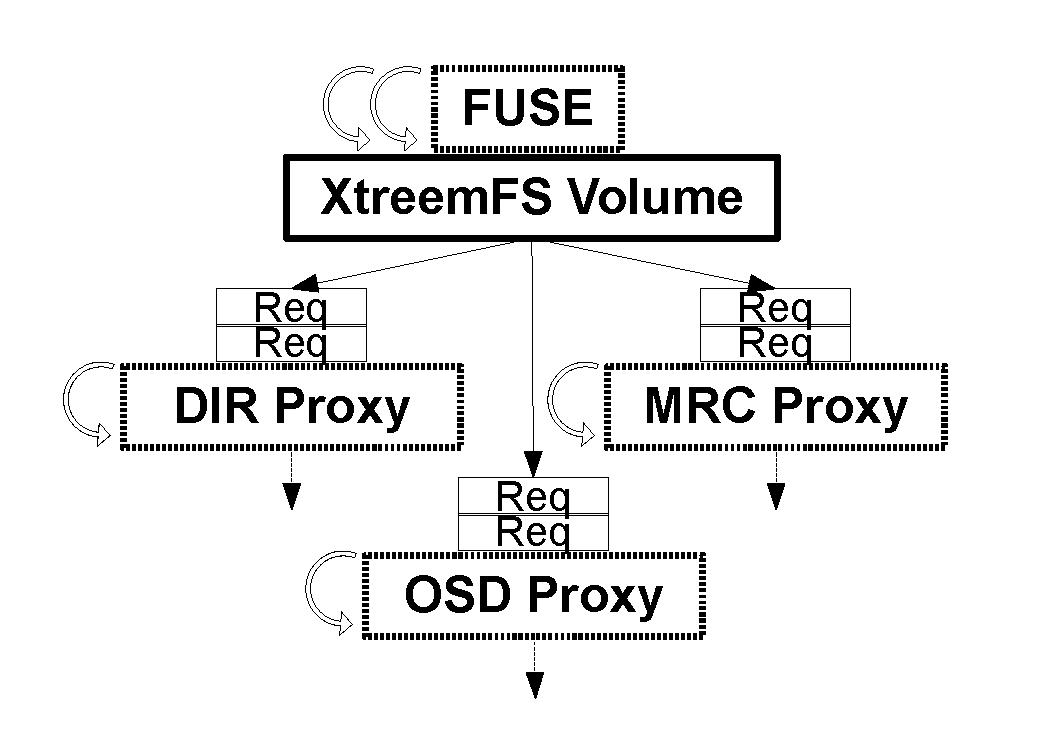
\includegraphics[width=.80\columnwidth]{images/xtreemfs_client_stages}
\caption{Client stages}
\label{xtreemfs_client/figures/xtreemfs_client_stages}
\end{figure}

\subsubsection{FUSE\index{FUSE}}

\texttt{xtfs\_mount} provides a file system interface to applications via FUSE\index{FUSE} \footnote{\url{http://fuse.sourceforge.net/}}, a library for implementing file systems in userspace. Applications make POSIX\index{POSIX} system calls such as \texttt{open} and \texttt{read} into the operating system kernel. A FUSE\index{FUSE} kernel module translates these calls into messages (i.e. Remote Procedure Calls), which are then passed to a FUSE\index{FUSE} file system via a pipe. The file system runs as a daemon in an infinite loop, reading and processing messages from the pipe and sending responses back into the kernel. The userspace part of the FUSE\index{FUSE} library handles most of the nitty gritty details of kernel-userspace communication, so that the file system implementator can concentrate on implementing file system logic. This is typically done by implementing a set of FUSE\index{FUSE} callbacks, each of which corresponds to a POSIX\index{POSIX} system call (and thus a message on the FUSE\index{FUSE} pipe as well). The FUSE\index{FUSE} library translates messages to calls on the callbacks supplied by the file system developer and translates return values from the callbacks back into messages for the FUSE\index{FUSE} kernel module. These FUSE\index{FUSE} callbacks are the main entry points into \texttt{xtfs\_mount}.

From a FUSE\index{FUSE} callback such as \texttt{mkdir} the client makes a series of requests (messages) through the various stages shown in figure \ref{xtreemfs_client/figures/xtreemfs_client_stages}. The primary stages in the client are proxies for the servers the \texttt{xtfs\_mount} instance is connected to: typically a single DIR server and a single MRC\index{MRC} server and multiple OSD\index{OSD} servers. In the case of \texttt{mkdir} the client would send a request to the \texttt{MRCProxy} to create the specified directory. Because the FUSE\index{FUSE} callbacks are synchronous the initial request from a callback to a stage must be synchronous, i.e. the sender must wait for the response before doing any further processing. However, this does not mean that the whole system is synchronous: only the FUSE\index{FUSE} callback blocks synchronously on a request, allowing the stages in the client to communicate asynchronously (and thus improve performance). Furthermore, since the FUSE\index{FUSE} callbacks may be multithreaded and reentrant a stage (such as e.g. the \texttt{MRCProxy}) can process requests from multiple FUSE\index{FUSE} callbacks simultaneously. In other words, the concurrency of the client is not limited by the FUSE\index{FUSE} front end and the number of threads processing FUSE\index{FUSE} messages.

\subsection{Implementation}

The XtreemFS client is implemented entirely in C++. Aside from the essential components listed above (FUSE\index{FUSE} callbacks, server proxies) \texttt{xtfs\_mount} consists of a few support classes such as \texttt{Path} (which wraps XtreemFS \texttt{volume\/file} global paths) and XtreemOS integration code such as a pluggable module for retrieving user credentials from an XtreemOS AMS server. Most of this code is shared between the XtreemFS command line tools listed in table \ref{xtreemfs_client/tables/command_line_tools}. As mentioned previously, the XtreemFS client also relies heavily on Yield for many low-level classes, such as platform-specific file paths and sockets. The ONC-RPC \cite{RFC1831} protocol implementation used to communicate with the XtreemFS servers is also a part of Yield. 

\subsubsection{Generated interfaces}

The synchronous request-response messages exchanges between FUSE\index{FUSE} callbacks and stages such as the \texttt{MRCProxy} are hidden underneath a function call interface. The latter is generated from the same IDL\index{IDL} interfaces used by the server. When one of the interface operations is called synchronously on the \texttt{MRCProxy} a request is created and filled with the function parameters; the request is sent to the \texttt{MRCProxy} stage, where it is processed asynchronously; and the caller blocks waiting for the response, which, when it is received, is unpacked and returned as a normal function return value. The extra level of abstraction allows the FUSE\index{FUSE} callback interface to be fully agnostic of message sending and receiving, and simply treat the MRCProxy as if it were making synchronous remote procedure calls. The FUSE\index{FUSE} callback for \texttt{mkdir} is shown in figure \ref{xtreemfs_client/figures/xtreemfs_client_mkdir_code}.

\begin{figure}[h!]
\begin{verbatim}
bool Volume::mkdir( const YIELD::Path& path, mode_t mode )
{
  mrc_proxy.mkdir( Path( this->name, path ), mode );
  return true;
}
\end{verbatim}
\caption{FUSE\index{FUSE} callback for mkdir}
\label{xtreemfs_client/figures/xtreemfs_client_mkdir_code}
\end{figure}

\subsubsection{Lines of code}

With much of its low-level functionality in Yield and other libraries the code base for the XtreemFS client is quite minimal, with approximately 2800 lines of hand-written C++ and 4800 lines of C++ automatically generated from the XtreemFS IDL\index{IDL} interfaces.

%MSC
\chapter{RMS - Replica Management Service}
\label{sec:xtreemfs_rms}

One of the most important mechanisms in XtreemFS is the possibility to have
several replicas of a file distributed over the Grid. This feature affords
data-intensive applications achieving better performance as long as: there is no
single access point for the data and mechanisms for parallel access can be
exploited. Besides, replication also provides reliability and availability to
the filesystem, which is of vital importance for a distributed environment.

However, the usage of Grid resources such as network (where data is transfered
across) or storage (where data is stored) are finite, shared, and non-free.
Furthermore, the synchronization of the replicas of any given file involves
additional overheads, so that mechanisms that keep the tradeoff between the
benefits and the extra costs are needed.

For aiming at all of these purposes, we are working on the implementation of the
Replica Management Service. This service concerns about: selecting the best
replicas for the applications, creating and deleting replicas automatically
taking account of how and from where they are accessed and evaluating the
maximum number of replicas of any given file.


\subsection{Choosing the best replica}
\label{RMS_Choosing_Replicas}

When a given client (or an OSD) has to access a file, the question is: which
replica should it access? It should be able to detect which replica will provide
better performance. The idea to solve this problem is to build a virtual 2D
space and locate all replicas, OSDs, and clients in it. The distance
between two different objects (i.e replica, OSD, or client) is an indicator of
the distance (performance wise) of these two objects. Once a client wants to
access a file, it just needs to compute the euclidian distance between itself
and all replicas and choose the closer one.

\subsubsection{Vivaldi Algorithm}

Vivaldi is a light-weight algorithm developed by MIT \cite{dabek2004vdn} 
that allows assigning a position in a coordinate space to every node in a network,
so the distance between the coordinates of two nodes predicts the real communication
latency between them.

In order to generate a valid coordinate system, it is necessary to determine
which space will be used and which formula will be used to calculate the
distance between two given points. In our case, it is been proved that
implementing a 2-D space, where the Euclidean distance between two coordinates
accurately predicts the latency between their corresponding nodes, generates
valid results with a really small error probability.

For the algorithm to work correctly, it is also necessary that the nodes of the
system keep contacting themselves randomly and indefinitely to re-adjust their
position, so any possible change in the network may be reflected. In each
re-adjustment, a node contacts a different neighbor, gets its coordinates and
modifies its own coordinates, so eventually the Euclidean distance is as similar
as possible to the measured round trip time.

On the other hand, once a group of nodes have established a valid coordinate
system, it is necessary to use some mechanism that helps to reduce the impact of
introducing new nodes, so we avoid them to alter the already stabilized system.
That is why Vivaldi keeps in every node, besides the coordinates, a local error
that informs about how sure a node is about its position. This way, a node with
a steadier position will have a smaller local error and will influence more the
rest of nodes when they contact it to readjust their position (figure
\ref{rms1}).

\begin{figure}[t]
\begin{center}
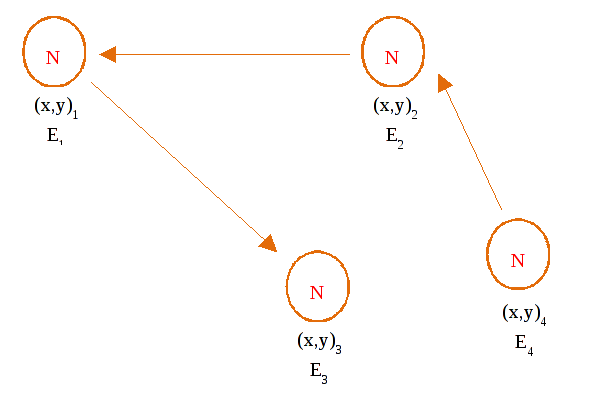
\includegraphics[width=0.60\textwidth]{images/rms1.png}
\caption{Nodes keep recalculating their position}
\label{rms1}
\end{center}
\end{figure}

Once the system is adjusted, any node of the network can determine which nodes
are the closest ones with a really simple calculation, in a very short period of
time and without generating extra traffic.

Some already developed implementations of Vivaldi can be found in p2psim and in
Chord. You might also be interested in Ledlie et al.'s work \cite{ledlie2007ncw}.

\subsubsection{Vivaldi in XtreemFS}

As we have different kinds of nodes in our architecture, not all of them work in
the same way to integrate Vivaldi. While the clients usually execute during
shorter periods of time, the servers are up and running , so the
idea is to let the OSDs (at this moment they are the only
servers that implement Vivaldi) establish a permanent coordinate system where a
client can move through, to find its position.

\subsubsection{Vivaldi in the OSDs}

An OSD has an independent stage responsible of managing Vivaldi on its side and
of providing to the rest of components a couple of valid coordinates that define
the position of the node in the current coordinate system.

The stage keeps running indefinitely and periodically contacts a different OSD
to ask it for its coordinates and its local error. With that data and the
coordinates of the own OSD is possible to compute the Euclidean distance and to
compare it with the real RTT measured against the contacted node.

The frequency an OSD readjusts its position is defined by the parameters
MIN\_\-TIMEOUT\_\-RECALCULATE and MAX\-\_TIMEOUT\_\-RECALCULATE. Just after performing a
readjustment, the stage typically calculates a random number included in the
interval of time defined by those two parameters and sleeps during that number
of seconds until the next iteration. This way we try to avoid generating traffic
peaks where all the nodes send a request at the same time and to distribute the
net use in time.

Larger periods will reduce the overhead in the network but will make the nodes
to adjust more slowly to the possible changes in the environment, while smaller
ones will require more traffic but will produce a more reactive system.

In each iteration, the introduced stage chooses a node to contact to from a list
of available OSDs, which is filled with the information contained in the
Directory Service. This list must be updated somehow so the stage can always
notice a node going offline.

\subsubsection{Vivaldi in clients}

In our system, the clients usually execute during a much shorter period of time,
so they have to be able to determine their position faster. This can be done
because they do not influence the rest of the nodes and they just take some
needed info from the already placed OSDs to locate themselves.

In Vivaldi, each node is responsible for its own coordinates and typically has to
recalculate them at least a small number of times before they represent the real
position in the coordinate system. Even if the set of OSDs is``adjusted'', a
client will need to recalculate its position (against one single node each time)
several times before having an accurate approximation of its real location.
Vivaldi requires that the nodes of the net generate traffic and communicate
among themselves.

As in the case of the OSDs, a client also has the parameters
MIN\_\-TIMEOUT\_\-RECALCULATE and MAX\_\-TIMEOUT\_\-RECALCULATE that allow defining the
recalculation period. Although the analogue parameters in the OSDs have the same
names, they are different parameters and therefore they all must be defined in
different files.

Finally, it is important to emphasize that after the first boot of the client,
it keeps its coordinates and preserves them among executions, so it remains well
located though it mounts and unmounts a lot of different volumes or opens and
closes a lot of files. The coordinates are not reinitialized until the client
node is rebooted.

\subsubsection{Replica Selection with Vivaldi}

Until this point we have introduced a mechanism able of establishing a
coordinate system where all the nodes of a network have a pair of coordinates
that allows them predicting the round trip time to the rest of neighbors. Now it
is time to analyze how to take advantage of that information and to describe the
current applications of Vivaldi in XtreemFS.

Sometimes during the execution of certain operations, the client has to choose
which replica access, among several replicas stored in different nodes of the
system. The ideal solution proposes to select always the replica that is stored
in the closest node, so the accesses can be made within the minimum time. But
the problem is that most of the times measuring the RTT against every OSD, for
each selection, is not computationally feasible.

Using the coordinates provided by Vivaldi, a client can calculate which replica
is the closest one with a practically insignificant delay. At this point the
only remaining problem seems to be how to gather all the coordinates so they can
be available in the exact moment of the replica selection.

As mentioned earlier, in Vivaldi the coordinates are managed
independently by the node they belong to and remain distributed among the
different nodes of the network. In order to let the client take advantage of
them, it is necessary to collect them in the MRC, so they can be included in
every list of x-locations.

\begin{figure}[t]
\begin{center}
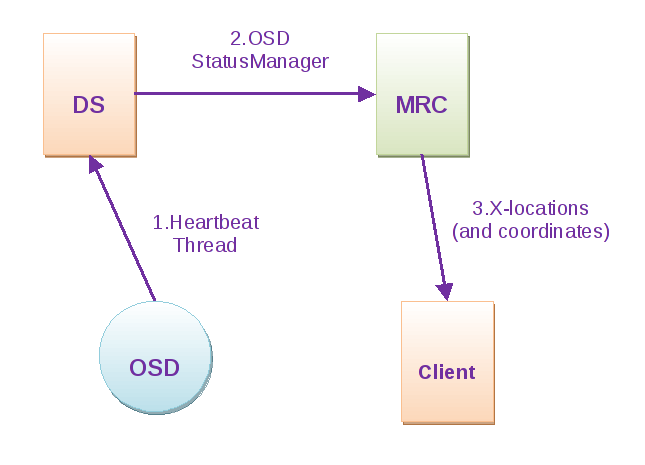
\includegraphics[width=0.60\textwidth]{images/rms2.png}
\caption{Collecting the coordinates}
\label{rms2}
\end{center}
\end{figure}

In figure \ref{rms2} we show the following process:

\begin{enumerate}
\item HeartbeatThread is a component of the OSDs that periodically registers the
OSD in the Directory Service. The information that is uploaded each time is
determined by the function getServiceData, which is defined in the main
constructor of the class OSDRequestDispatcher.
\item OSDStatusManager is a component of the MRC that regularly queries the
Directory Service for available OSDs.
\item During an open operation, the MRC sends to a client a list of x-locations,
so it can locate the different replicas associated to a certain file. The
x-locations include the corresponding coordinates, so the client can use them to
predict the closest replica.
\end{enumerate}


\subsection{Replica creation}
\label{RMS_Replica_Creation}

Another important issue regarding replicas is to decide when and where to create
a replica. For this functionality we have three different mechanisms. The first
one is an explicit request from the user. In this scenario, the RMS will not
take any action. The second one is a reactive replica creation. The system will
detect that a replica is needed at a given location and will start a replica
creation. Finally, in the third case, the system will predict the usage of a
file in a location where no replicas are nearby and thus will try to create the
replica before it is used. We call to this third mechanism proactive replica
creation.

In both cases reactive and proactive, we plan to provide a mechanism able to
study the access pattern of files and use it to decide if only a part of the
file needs to be replicated (partial replication). This partial replicas will
speedup the process of replication because only part of the data will need to be
copied to the new location. Nevertheless if we miss-predict the parts of the
replica that will be used, we will always be able to populate the missing parts
on-demand (done directly by the OSDs).

%TODO: We could increase the level of detail in following subsubsections
\subsubsection{Reactive replica creation with Vivaldi} 

In this scenario it is detected when replicas are currently needed in other
parts of the Grid. Then, using the distance mechanisms we just described in
Section \ref{RMS_Choosing_Replicas}, we will detect if clients request a replica
from large distances. So in this case Vivaldi could be used to decide a better
location for a replica and create it.

\subsubsection{Proactive replica creation with Oraculo}

We have implemented a service called Oraculo that carries out data mining on
multi-order context models to analyze the file-access patterns and to compute
future accesses. For the implementation of such multi-order context models,
Oraculo keeps a trie (or prefix tree) as Kroeger et al. did \cite{kroeger1996pfs,
kroeger2001dai} for centralized environments, where they proved that such structures
where effective. 

Thus, each file access is modeled as a symbol (i.e. the file path) and it is
recorded as a node of the prefix tree with an associated value that represents
how many times the chain pattern from root to that node has ocurred.

Then, in order to interact with Oraculo, it provides a basic interface for:
\begin{enumerate}
 \item Adding an event to the trie, given a sequence of the last events seen.
 \item Getting a prediction from the trie, given a sequence of the last events
seen.
\end{enumerate}

So that when a file access is produced, it can be noticed to Oraculo which
computes which parts of the trie must be modified, adding the new event to the
corresponding branches or simply increasing the counter of the pattern if it is
already present.

Notice that in order to keep the trie scalable Oraculo can prune it in two ways.
First, keeping a predefined maximum number of nodes per branch. Thus, whenever a
new event goes to a full branch all its nodes divide their corresponding value
by two and nodes with a value lower than 1 are deleted from the trie. In the
case that no node has been cleaned, the new event is not added. But, obviously
the nodes in the branch keep the new value (after the division by two) so in the
near future it will be eventually possible to add new events in that branch.

On the other hand, Oraculo also has a maximum of root-branches (also called
partitions) to keep the horizontal scalability of the trie. Here we apply a
LRU-based algorithm among the partitions taking account of their usage as well.

Finally, Oraculo can predict future file accesses by applying basic data-mining
on the trie. It only needs to know some previous accesses to look for patterns
based on them. Then, an OSD could eventually use this information to replicate
data in advance.

Furthermore, we will propose a decoupled and off-line aggregation of the tries.
Once in a while (still to be determined), OSDs could contact other OSDs (only a
small subset) to exchange their trie information and build an aggregated one
that has the information of all. This mechanism will allow all OSDs to have a
more or less global view because what is learned by one OSD will be propagated
though several aggregations. We have done some preliminary tests using this
mechanism and seems to work very well with environments of many thousands of
nodes.

Regarding the information of the access pattern of files, in most cases the
information kept by a single OSD will be enough. Nevertheless, whenever we need
the full information of the pattern, we can contact all OSDs that have a replica
and aggregate the learned behavior. As we do not expect to keep many replicas of
a file, this procedure seems reasonable and scalable.

\subsubsection{Integration of Oraculo with OSDs}

Unfortunately, the integration of Oraculo with OSDs could not be done yet
because we are still evaluating it by using GridSim (a well-known Grid
simulator). Once we get significant results with the simulations we will
evaluate them and port Oraculo to the OSDs.


%%WARNING: This subsection is copy pasted from D3.4.4
%\subsection{Automatic setting of the number of replicas}
%\label{RMS_replica_limitation}

%The problem of having many replicas is that updates imply that a coordination
%mechanisms has to be started. This coordination will reduce performance and the
%magnitude clearly depends on the number of replicas available. For this reason
%we have decided to set a limit in the number of replicas a file will have.

%On the other hand, it is clear that the overhead this coordination will imply
%also depend on the frequency at which files are modified. For instance, if a
%file is only modified once a month (and only small modification are done) we
%could keep many more replicas than for a file that is constantly modified.

%The objective of this mechanism is to detect the access pattern of files and
%find the ratio between reads and writes. With this information the RMS will
%decide the maximum number of replicas that obtains a good tradeoff between the
%benefit of multiple replicas in read operations and the penalty of coordination
%in write operations.


%%WARNING: This subsection is copy pasted from D3.4.4
\subsection{Replica deletion}
\label{RMS_Replica_Deletion}

On the one hand, if we want to be able to replicate files whenever needed but
still maintain the maximum number for replicas per file, it would be interesting
to keep the number of replicas a bit smaller than the maximum. This difference
between the maximum and the real number of replicas would allow the system to
create replicas whenever needed. On the other hand, if replicas are not used, it
would also be nice to have them removed automatically to reduce disk usage in a
given node and/or center.

To tackle these two issues we will implement a mechanism that automatically
deletes the less important replicas. To know what replicas are less important we
will use similar mechanisms than the ones used to create replicas. We will
predict future usage using the same kind of tries. In addition we will perform
some kind of preventive removal of replicas, which means that whenever a node
decides to remove a replica it will inform other OSDs that have it to react
accordingly.


%%WARNING: This subsection is copy pasted from D3.4.4
\subsection{Interaction with the Application Execution Management}
\label{RMS_AEM_interaction}

The last mechanisms that we will implement to manage replicas consists of an
interaction with the application execution management system (AEM). This
interaction will be done in two steps.

Firstly, AEM analyzes the JSDL of the application and asks to XtreemFS
for the locations (coordinates X,Y) of its files' references. Thus AEM computes
an optimal coordinate around where the job should be executed. This coordinate
is used for AEM to send a request to Resource Selection Service (RSS) for a set
of nodes close to it. Of course, RSS also considers other requirements, such as
CPU or memory, to decide the resulting set of nodes.

In the second step, the AEM will inform XtreemFS on the final destination of a
given job and the files it will use. With this information, the RMS will decide
if new replicas need to be created to improve the I/O performance of this job.
In addition, and in some cases, it might be that the RMS decides to advance this
step from the information obtained in step 1. For instance, this may happen when
the list is made of nodes that are close among themselves and one or two
replicas could do the job.

Although this mechanism is very good in the sense that no prediction needs to be
done, it has a couple of limitations. The first one is that the AEM might not
know the files used by a job (it is not a requirement in the job description).
The second one is that there might not be enough time from the moment XtreemFS
receives the execution location of a job (and the files it uses) and the moment
the job starts running. To solve these two cases we have proposed the previous
prediction mechanisms (\ref{RMS_Replica_Creation}).


%CNR, BSC
\chapter{Testing}
\label{sec:xtreemfs_test}
Regular and extensive testing is of vital importance for any file
system, in order to improve its reliability, scalability, code
quality, stability, performance, etc. Therefore, a new activity
inside the WP3.4 has been created, which is focused on all the
aspects of testing. The goal of this task is to evaluate
functionality and performance of XtreemFS, by exploiting some
existing file system test suites.

Nowadays, from a software viewpoint, there are some available tools
that are mainly designed for testing local file systems, but there
are no ready-made tools available for testing Grid File Systems.
Thus, in order to test XtreemFS, either some ad-hoc tools must be
developed or some existing distributed testing tools must be
extended.

Currently, there are two main guidelines leading the tests performed
on XtreemFS: the first one is aimed at evaluating the POSIX
compliance of XtreemFS and consequently its functionality; the
second one addresses the performance evaluation by stressing
XtreemFS with a set of tests and benchmarks (in the following we
refer to such kind of tests as regression tests).

In the next subsections we will describe both such activities, the
tools used and the results obtained.

\subsection{Testing POSIX compliance of XtreemFS}
One of the goals of XtreemFS is providing a POSIX-compliant
filesystem. In order to evaluate the correctness of functionalities,
we initially evaluated some available test suites aimed at the POSIX
compliance testing. Firstly, we evaluated the "Open Posix Tests
Suite" (https://sourceforge.net/projects/posixtest/); it resulted
not very suitable for our tests, because it performs only AIO tests
but nothing else related to the file system; moreover, we
encountered some difficulties during the installation and in
particular during the execution of the tests, and for such reasons
we discarded it. A second tool that we evaluated was the NTFS-3G
suite (http://www.ntfs-3g.org), that is a test suite available for
the most important operating systems; it includes a POSIX filesystem
test environment, the Pawel Jakub Dawidek's POSIX filesystem test
suite, that immediately seemed more suitable for our purposes than
the first one. For such a reason, we chose to exploit the PJD's
POSIX filesystem test suite (PJD-fstest) and to run it over
XtreemFS. The test suite is available on the Web under a BSD license
and we got it from http://www.ntfs-3g.org/pjd-fstest.html.
PJD-fstest performs almost 3700 regression tests that exhaustively
check a wide amount of different scenarios for the following system
calls:
\begin{itemize}
\item \textit{chmod}: changes the permissions of a files or directories
\item \textit{chown}: changes the owner of files or directories
\item \textit{link}: creates hard link
\item \textit{mkdir}: creates directories
\item \textit{mkfifo}: creates fifo named pipes
\item \textit{open}: opens a file
\item \textit{rename}: renames files or directories
\item \textit{rmdir}: removes directories
\item \textit{symlink}: creates symbolic links
\item \textit{truncate}: truncates files
\item \textit{unlink}: removes files
\end{itemize}

For each system call, the suite contemplates the execution of a set
of scripts. Each script performs a set of basic operations, like the
creation of a directory, the change of its access rights, the change
of its owner, etc., and for each operation it evaluates its return
value. If such a value is different than that expected, an error is
pointed out. Obviously, the scripts performing the tests for a
particular system call are composed of operations targeted for the
evaluation of the (hopefully correct) behaviour of that system call.
Our work consists in the automatic execution of the scripts and in
the evaluation of the failure events. Then, for each failure, we
need to interpret the cause of the problem and reproduce manually
the scenario (the sequence of operations) causing it. After this
step (that some time hides some difficulties) the problem is pointed
out in a bug tracker, in order to be scheduled for a solution.

\subsubsection{How to execute the tests}

After downloading the tarball of the PJD-fstest, we can simply extract its contents:

\verb"tar xvzf <package>"

The most significant contents of the tarball are:

\begin{itemize}
\item \textit{fstest.c}: the source code
of the main program. It provides an implementation of all the syscalls commented before.
\item \textit{Makefile}: the Makefile that we can use to compile the program.
\item \textit{tests}: a directory that contains one subdirectory for every syscall.
For each of this subdirectories, there is a set of scripts that conform the tests for the corresponding syscall.
\end{itemize}

Afterwards, we can compile the fstest.c file by executing \textbf{\textit{make}}.

To execute the tests, we have implemented a tool that basically
automatizes all  the process of updating, compiling, and installing
XtreemFS, running a basic scenario with one Directory Service, one
MRC and an OSD, and creating a volume and mounting it on a specific
directory.

Once this scenario is up and running, we enter the mount-point where
the volume  is mounted and execute the tests by using the command
\textbf{\textit{prove}} as follows:

\verb"sudo prove -r <path_to_pjd_suite>/tests"

The flag \textit{-r} specifies that \textit{prove} should traverse
all the directories recursively (so all the tests are executed).
Notice that we need root privileges so we also need to edit
\textit{/etc/fuse.conf} and add the following line:

\verb"user_allow_other"

This line allows non-root users to specify the option
\textit{allow\_other} (or \textit{allow\_root})  among the mounting
options of fuse.


\subsubsection{Results}

At the moment, XtreemFS does not support fifos, so mkfifo tests are being ignored.

The tests corresponding to the rest of the syscalls were executed
completely and the only errors encountered were due to the lack of
implementation of sticky bits on files and directories.

We plan to work on it in next XtreemFS versions, although it is not
a very  important feature and currently we have to spend our efforts
on other more significant issues.


\subsection{Regression Tests}
We use a set of regular file system test tools and custom made tests to automatically check the XtreemFS development version (the svn trunk) every night. This test environment can also be used to manually run these tests.

The main test script is \texttt{trunk/bin/xtfs\_test} and can be executed to run all tests automatically or to start/stop a test environment.

To start a test environment with all XtreemFS servers and clients, run

\begin{verbatim}
 > trunk/bin/xtfs_test --start
\end{verbatim}

This script will put all data and logfiles in the current working directory.

After setting up the test environement, the tests in \texttt{trunk/tests/} can be executed individually by calling the test scripts in the mounted XtreemFS volume.

\begin{verbatim}
 > python trunk/tests/01_simple_metadata.sh
\end{verbatim}

To shutdown all servers and unmount the clients after testing, execute

\begin{verbatim}
 > trunk/bin/xtfs_test --stop
\end{verbatim}

To clean up all data and logfiles use

\begin{verbatim}
 > trunk/bin/xtfs_test --clean
\end{verbatim}

If you want to run all tests automatically, run the test script in auto mode

\begin{verbatim}
 > trunk/bin/xtfs_test --autotest
\end{verbatim}


%ZIB, NEC
\chapter{Protocol and Interactions}
\label{sec:xtreemfs_proto}






XtreemFS uses ONC RPC\cite{RFC1831}\index{ONC RPC} for executing remote operations. Interfaces and records are defined in a subset of CORBA IDL\index{IDL}. Yidl\footnote{http://code.google.com/p/yield/} is used to generate the code for the interfaces and records in C++ and Java.

To build the Java classes from the interfaces:
\begin{enumerate}
 \item export \texttt{PYTHONPATH} to point to your yidl source directory:\\
       \texttt{export PYTHONPATH=/home/user/yidl/src}
 \item execute \texttt{bin/generate\_xtreemfs\_java.py}
\end{enumerate}


\makeatletter
\renewcommand\paragraph{\@startsection{paragraph}{4}{\z@}%
  {-3.25ex\@plus -1ex \@minus -.2ex}%
  {0.1ex \@plus .0ex}%
  {\normalfont\normalsize\bfseries}}
\makeatother

\subsection{Constants}
\label{sec:xtreemfs_proto_const}

Globally shared constants are defined in \texttt{in\-ter\-faces/const\-ants.idl}.

\begin{description}
	\item[\texttt{ACCESS\_CONTROL\_POLICY\_NULL}] don't use any access policy (on the MRC\index{MRC}). This will allow all users to do everything on the volume.

	\item[\texttt{ACCESS\_CONTROL\_POLICY\_POSIX}] use standard POSIX\index{POSIX} permissions (user, group, others) on the volume.

	\item[\texttt{ACCESS\_CONTROL\_POLICY\_VOLUME}] similar to POSIX\index{POSIX} permissions but the permission for the root (/) is used for the entire volume.

	\item[\texttt{ACCESS\_CONTROL\_POLICY\_DEFAULT}] the policy to use in e.g. mkvol if nothing is specified.

	\item[\texttt{ONCRPC\_SCHEME}] scheme for URLs.

	\item[\texttt{ONCRPCS\_SCHEME}] scheme for URLs when using SSL.

	\item[\texttt{ONCRPC\_AUTH\_FLAVOR}] constant to use for ONC RPC\index{ONC RPC} auth\_flavor to indicate XtreemFS auth. If present, a UserCredentials record is sent in auth\_opaque

	\item[\texttt{OSD\_SELECTION\_POLICY\_SIMPLE}] only OSDs which are alive and which have more than 2GB free space are used.

	\item[\texttt{OSD\_SELECTION\_POLICY\_DEFAULT}] the policy to use in e.g. mkvol if nothing is specified.

	\item[\texttt{REPL\_UPDATE\_PC\_NONE}] no replication is used

	\item[\texttt{REPL\_UPDATE\_PC\_RONLY}] read-only replication

	\item[\texttt{SERVICE\_TYPE\_MRC}] for DIR\index{DIR} service registry, service is an MRC\index{MRC}

	\item[\texttt{SERVICE\_TYPE\_OSD}] for DIR\index{DIR} service registry, service is an OSD\index{OSD}

	\item[\texttt{SERVICE\_TYPE\_VOLUME}] for DIR\index{DIR} service registry, service is a volume

	\item[\texttt{STRIPING\_POLICY\_RAID0}] RAID0 (striping)

	\item[\texttt{STRIPING\_POLICY\_DEFAULT}] the policy to use in e.g. mkvol if nothing is specified.

	\item[\texttt{STRIPING\_POLICY\_STRIPE\_SIZE\_DEFAULT}] default stripe size in KB to use if nothing is specified.

	\item[\texttt{STRIPING\_POLICY\_WIDTH\_DEFAULT}] default striping width (number of OSDs\index{OSD}) to use if nothing is specified.

	\item[\texttt{SYSTEM\_V\_FCNTL\_H\_O\_...}] POSIX\index{POSIX} constants

\end{description}

\subsection{Types}

\subsubsection{Globally Shared Types}

Globally shared data structures are defined in \texttt{inter\-faces/types.idl}.

\paragraph{\texttt{struct UserCredentials}}

User information sent in the ONC RPC\index{ONC RPC} \texttt{opaque\_auth} body if XtreemFS authentication is used. How the userID and groupIDs look like depends on the policy used in the client which translates the local uid/gid.

\begin{tabularx}{\textwidth}{lX}
 \texttt{user\_id} & globally unique userID\\
 \texttt{group\_ids} & list of globally unique groupIDs (must contain at least one entry)\\
 \texttt{password} & admin password (in cleartext) required for some operations (e.g. mkvol)
\end{tabularx}

\paragraph{\texttt{struct VivaldiCoordinates}}

Structure used to exchange Vivaldi coordinates between components, also used in UDP\index{UDP} packets for measuring latency between XtreemFS clients and OSDs\index{OSD}.

\begin{tabularx}{\textwidth}{lX}
 \texttt{x\_coordinate} & x coordinate\\
 \texttt{y\_coordinate} & y coordinate\\
 \texttt{local\_error} & confidence in correctness of x/y coordinates
\end{tabularx}


\subsubsection{Types Shared between MRC\index{MRC} and OSD\index{OSD}}

Types that are mainly shared between MRC\index{MRC} and OSD\index{OSD} are defined in \texttt{inter\-faces/mrc\_osd\_\-types.idl}.

\paragraph{\texttt{struct NewFileSize}}
Sent by the OSD\index{OSD} in response to a file modification operation if the file size has changed. A client may cache these updates and send them to the MRC\index{MRC} when renewing a capability, on fsync/flush and close. The client needs only to send the most recent record it received from the OSD\index{OSD} for a given file. Most recent means that: \texttt{
(size\_in\_bytes' $>$ size\_in\_bytes} \texttt{AND} \texttt{truncate\_epoch' == truncate\_epoch) 
OR} \texttt{(truncate\_epoch' $>$ truncate\_epoch)}

The client should update its local file size cache with the NewFileSize records received from the OSD\index{OSD}. The client should use the \textit{locally cached} file size on stat rather than the result from the MRC\index{MRC} to ensure that local processes see their own modifications.

\begin{tabularx}{\textwidth}{lX}
 \texttt{size\_in\_bytes} & the new file size in bytes\\
 \texttt{truncate\_epoch} & truncate epoch in which this operation was executed (used by the MRC\index{MRC} for ordering updates)
\end{tabularx}


\paragraph{\texttt{struct OSDtoMRCData}}
Data sent by the OSD\index{OSD} to the client which is expected to pass it on to the MRC\index{MRC}. When the data should be passed to the MRC\index{MRC} depends on the \texttt{caching\_policy}. This feature is currently not used.

\begin{tabularx}{\textwidth}{lX}
 \texttt{caching\_policy} & describes how the client is allowed to cache the data (when to send it to the MRC\index{MRC})\\
 \texttt{data} & opaque data
\end{tabularx}

\paragraph{\texttt{struct OSDWriteResponse}}
Record containing file size updates and/or OSDtoMRCData. Returned from all data-modifying operations.

\begin{tabularx}{\textwidth}{lX}
 \texttt{new\_file\_size} & contains no record or at most one record if the file size changed\\
 \texttt{opaque\_data} & contains 0 or more records
\end{tabularx}


\paragraph{\texttt{struct StripingPolicy}}
Describes how a replica (one copy of the file) is split into objects.

\begin{tabularx}{\textwidth}{lX}
 \texttt{policy} & describes the scheme to use for distributing the objects among the OSDs\index{OSD}, e.g. RAID0 for simple round robin striping.\\
 \texttt{stripe\_size} & the size of the objects in kilobytes, must be $>= 4$\\
 \texttt{width} & the number of OSDs\index{OSD} to use for striping, must be $>= 1$.
\end{tabularx}


\paragraph{\texttt{struct Replica}}
Describes a single copy of a file.

\begin{tabularx}{\textwidth}{lX}
 \texttt{striping\_policy} & the striping policy to use for this replica.\\
 \texttt{replication\_flags} & value depends on the replication policy, e.g. to indicate a full or lazy replica.\\
 \texttt{osd\_uuids} & ordered (!) list of OSDs\index{OSD} holding objects of the file.
\end{tabularx}



\paragraph{\texttt{struct XLocSet}}
Describes a complete file together with all replicas (copies) and how they are kept consistent.

\begin{tabularx}{\textwidth}{lX}
 \texttt{replicas} & list of the file's replicas (i.e. list of Replica structs)\\
 \texttt{version} & incremented by the MRC\index{MRC} on each modification of the list. Used by the OSD\index{OSD} to reject clients working with outdated lists.\\
 \texttt{repUpdatePolicy} & the policy used for keeping replicas in sync. \\
 \texttt{read\_only\_file\_size} & the size of the file in bytes, used only for read-only replication.
\end{tabularx}


\paragraph{\texttt{struct XCap}}
Security token which is issued by the MRC\index{MRC} and authorizes a client to execute operations on a file at the OSDs\index{OSD}.

\begin{tabularx}{\textwidth}{lX}
 \texttt{file\_id} & file for which the capability can be used\\
 \texttt{access\_mode} & POSIX\index{POSIX} access mode for which client is authorized (e.g. read only, delete, write, truncate).\\
 \texttt{expires\_s} & absolute timestamp when the capability becomes invalid (seconds since epoch). \\
 \texttt{client\_identity} & the client identity set by the MRC\index{MRC}, currently the client's IP address. \\
 \texttt{truncate\_epoch} & the file's current truncate epoch. \\
 \texttt{server\_signature} & the MRC's\index{MRC} signature for the capability which is used by the OSD\index{OSD} to validate the XCap. Signature is created using shared secret specified in the MRC\index{MRC} and OSD\index{OSD} configuration. \\
\end{tabularx}



\paragraph{\texttt{struct FileCredentials}}
A record containing the XLocSet and XCap for a file. Required for most OSD\index{OSD} operations.

\begin{tabularx}{\textwidth}{lX}
 \texttt{xlocs} & the XLocSet\\
 \texttt{xcap} & the capability\\
\end{tabularx}


\paragraph{\texttt{sequence<FileCredentials> FileCredentialsSet}}
Used by the MRC\index{MRC} to return no or at most one FileCredentials record.





% %%%%%%%%%%%%%%%%%%%%%%%%%% EXCEPTIONS %%%%%%%%%%%%%%%%%%%%%%%%%%%%%%%%%
\subsubsection{Exceptions}

Exceptions that may be thrown in connection with an RPC are defined in \texttt{interfaces/exceptions.idl}.

\paragraph{\texttt{exception ProtocolException}}
Thrown on ONC RPC\index{ONC RPC} errors (e.g. GARBAGE\_ARGS)

\begin{tabularx}{\textwidth}{lX}
 \texttt{accept\_stat} & ONC RPC\index{ONC RPC} \texttt{accept\_stat} value\\
 \texttt{error\_code} & POSIX\index{POSIX} errno, if available\\
 \texttt{stack\_trace} & optional, for debugging only
\end{tabularx}


\paragraph{\texttt{exception errnoException}}
Thrown by the MRC\index{MRC} to indicate a POSIX\index{POSIX} error.

\begin{tabularx}{\textwidth}{lX}
 \texttt{error\_code} & POSIX\index{POSIX} errno, if available\\
 \texttt{error\_message} & optional text message\\
 \texttt{stack\_trace} & optional, for debugging only
\end{tabularx}


\paragraph{\texttt{exception RedirectException}}
Thrown by the DIR\index{DIR},MRC\index{MRC} and OSD\index{OSD} to redirect the client to another service. Use e.g. for master slave replication to direct the client to the current master.

\begin{tabularx}{\textwidth}{lX}
 \texttt{to\_uuid} & service to contact\\
\end{tabularx}


\paragraph{\texttt{exception ConcurrentModificationException}}
Thrown by the DIR\index{DIR} if a record was modified by another service on the meantime.

\begin{tabularx}{\textwidth}{lX}
 \texttt{stack\_trace} & optional, for debugging only
\end{tabularx}


\paragraph{\texttt{exception InvalidArgumentException}}
Thrown by the DIR\index{DIR} if an input value is not acceptable.

\begin{tabularx}{\textwidth}{lX}
 \texttt{error\_message} & error message describing the correct values.
\end{tabularx}


% %%%%%%%%%%%%%%%%%%%%%%%%%% DIR INTERFACE %%%%%%%%%%%%%%%%%%%%%%%%%%%%%%%%%
\subsection{Directory Service Interface}

The Directory Service interface is defined in \texttt{interfaces/dir\_interface.idl}.

\paragraph{\texttt{struct AddressMapping}}
Maps a service UUID to protocol, hostname/IP and port. A service can have multiple mappings for different networks (e.g. inside a cluster with private IP addresses). At the moment only ``*'' is supported for \texttt{match\_network} which indicates a match for all networks.

\begin{tabularx}{\textwidth}{lX}
 \texttt{uuid} & the service UUID\\
 \texttt{version} & the record's version, used by the DIR\index{DIR} to detect concurrent modifications\\
 \texttt{protocol} & the protocol used by the service\\
 \texttt{address} & resolvable hostname or IP address in text form\\
 \texttt{port} & port on which the service listens\\
 \texttt{match\_network} & for future use, must be \texttt{*}\\
 \texttt{ttl\_s} & time to live in seconds, indicates how long this record can be cached before it is re-fetched from the DIR\index{DIR}\\
\end{tabularx}

\paragraph{\texttt{sequence<AddressMapping> AddressMappingSet}}
Future releases of XtreemFS will support multi-network setups to ease the usage of XtreemFS in shared public/private network environments often found in clusters.


\paragraph{\texttt{struct Service}}
Information on a service registered at the DIR\index{DIR}.

\begin{tabularx}{\textwidth}{lX}
 \texttt{uuid} & the service UUID\\
 \texttt{version} & the record's version, used by the DIR\index{DIR} to detect concurrent modifications\\
 \texttt{type} & service type (see \ref{sec:xtreemfs_proto_const})\\
 \texttt{name} & human readable name of the service; for volumes: the unique volume name\\
 \texttt{last\_updated\_s} & timestamp of the last time (in seconds since epoch) the service updated its entry at the DIR\index{DIR}. Used as a coarse-grained heartbeat-signal.\\
 \texttt{data} & a map of additional data which depends on the service (e.g. MRC\index{MRC} of a volume or free space of an OSD\index{OSD})\\
\end{tabularx}


\paragraph{\texttt{void xtreemfs\_address\_mappings\_get( string uuid, out AddressMappingSet address\_mappings~)}}
Get an address mapping for the service specified by \texttt{uuid}.

\begin{tabularx}{\textwidth}{lX}
 \texttt{uuid} & the service UUID\\
 \texttt{out address\_mappings} & empty, if no mapping exists, one (or more) records otherwise\\
\end{tabularx}


\paragraph{\texttt{void xtreemfs\_address\_mappings\_remove( string uuid~)}}
Remove an address mapping from the DIR\index{DIR}.

\begin{tabularx}{\textwidth}{lX}
 \texttt{uuid} & the service UUID\\
\end{tabularx}


\paragraph{\texttt{uint64\_t xtreemfs\_address\_mappings\_set( AddressMappingSet address\_mappings~)}}
Updates the address mappings for a service. 

\begin{tabularx}{\textwidth}{lX}
 \texttt{address\_mappings} & the new mappings. The UUID in all records must be the same. The version must be 0 for a new mapping or the version obtained with the last read from the DIR\index{DIR}.\\
 returns & the new version of the mapping\\
 throws & ConcurrentModificationException if the record was updated (version incremented by DIR\index{DIR}) between reading and updating the record.
\end{tabularx}


\paragraph{\texttt{void xtreemfs\_checkpoint()}}
Forces the DIR\index{DIR} to create a BabuDB checkpoint. This operation does not block, the checkpoint is created asynchronously. The admin password must be sent via the XtreemFS authentication.


\paragraph{\texttt{uint64\_t xtreemfs\_global\_time\_s\_get()}}
Returns the current system time on the DIR\index{DIR} in seconds since epoch. Used to synchronize MRCs\index{MRC} and OSDs\index{OSD} to the global XtreemFS system time. The DIR\index{DIR} system should be synchronized with a precise clock using e.g. ntp.

\begin{tabularx}{\textwidth}{lX}
 returns & system time in seconds since UNIX epoch.
\end{tabularx}


\paragraph{\texttt{void xtreemfs\_service\_get\_by\_type( uint16\_t type, out ServiceSet services~)}}
Get all services of a specific type registered at the DIR\index{DIR}.

\begin{tabularx}{\textwidth}{lX}
 \texttt{type} & the service type to return\\
 \texttt{out services} & all matching services\\
\end{tabularx}


\paragraph{\texttt{void xtreemfs\_service\_get\_by\_uuid( string uuid, out ServiceSet services~)}}
Get the service information for a service with a specific UUID.

\begin{tabularx}{\textwidth}{lX}
 \texttt{uuid} & the service uuid\\
 \texttt{out services} & one record, if the service is registered, empty list otherwise\\
\end{tabularx}


\paragraph{\texttt{void xtreemfs\_service\_get\_by\_name( string name, out ServiceSet services~)}}
Get the service information for a service with a specific name.

\begin{tabularx}{\textwidth}{lX}
 \texttt{name} & the service's name\\
 \texttt{out services} & one record, if the service is registered, empty list otherwise\\
\end{tabularx}



\paragraph{\texttt{uint64\_t xtreemfs\_service\_register( Service service~)}}
Update a service registration at the DIR\index{DIR}. Updates the \texttt{last\_update\_s} field of the service.

\begin{tabularx}{\textwidth}{lX}
 \texttt{service} & the service's data. The UUID must be the service's UUID, the version must be 0 for a new service or the version obtained with the last read from the DIR\index{DIR}.\\
 returns & the new version of the mapping\\
 throws & ConcurrentModificationException if the record was updated (version incremented by DIR\index{DIR}) between reading and updating the record.\\
\end{tabularx}


\paragraph{\texttt{void xtreemfs\_service\_deregister( string uuid~)}}
Removes the service registry entry for the service from the DIR\index{DIR}.

\begin{tabularx}{\textwidth}{lX}
 \texttt{uuid} & the service uuid\\
\end{tabularx}


\paragraph{\texttt{void xtreemfs\_service\_offline( string uuid~)}}
Sets the \texttt{last\_update\_s} field to 0 which indicates that the service was taken offline.

\begin{tabularx}{\textwidth}{lX}
 \texttt{uuid} & the service uuid\\
\end{tabularx}


\paragraph{\texttt{void xtreemfs\_shutdown()}}
Shuts down the DIR\index{DIR} service, does not force a checkpoint of the database. The admin password must be sent via the XtreemFS authentication.




% %%%%%%%%%%%%%%%%%%%%%%%%%% MRC INTERFACE %%%%%%%%%%%%%%%%%%%%%%%%%%%%%%%%%
\subsection{Metadata and Replica Catalog Interface}
\label{sec:mrc_interface}

The MRC\index{MRC} interface is defined in \texttt{interfaces/mrc\_interface.idl}.

\paragraph{\texttt{struct Stat}}
Contains information about a file, directory or symbolic link that is sent to the client in response to a \texttt{getattr} request.

\begin{tabularx}{\textwidth}{lX}
 \texttt{mode} & the file's current access mode\\
 \texttt{nlink} & the number of hard links to the file\\
 \texttt{uid} & the numeric UID of the file's owner (just for compatibility reasons, will not be filled)\\
 \texttt{gid} & the numeric GID of the file's owner (just for compatibility reasons, will not be filled)\\
 \texttt{unused\_dev} & (just for compatibility reasons, will not be filled)\\
 \texttt{size} & the current file size in bytes\\
 \texttt{atime\_ns} & the file's atime in nanos\\
 \texttt{mtime\_ns} & the file's mtime in nanos\\
 \texttt{ctime\_ns} & the file's ctime in nanos\\
 \texttt{user\_id} & the XtreemFS user ID string of the file's owner\\
 \texttt{group\_id} & the XtreemFS group ID string of the file's owner\\
 \texttt{file\_id} & the XtreemFS file ID\\
 \texttt{link\_target} & the target path for symbolic links\\
 \texttt{truncate\_epoch} & the file's current truncate epoch\\
 \texttt{attributes} & a set of Win32 specific file attributes\\
\end{tabularx}

\paragraph{\texttt{struct DirectoryEntry}}
Contains information about a directory entry that is sent to the client in response to a \texttt{readdir} request.

\begin{tabularx}{\textwidth}{lX}
 \texttt{name} & the name of the directory entry\\
 \texttt{stbuf} & a buffer of type \texttt{struct Stat} that contains information about the file\\
\end{tabularx}

\paragraph{\texttt{struct StatVFS}}
Contains information about a mounted XtreemFS volume, which is sent to the client in response to a \texttt{statvfs} request.

\begin{tabularx}{\textwidth}{lX}
 \texttt{bsize} & the file system's block size (1024)\\
 \texttt{bfree} & the number of free blocks\\
 \texttt{fsid} & the file system ID (volume ID)\\
 \texttt{namelen} & maximum file name length (1024)\\
\end{tabularx}

\paragraph{\texttt{struct Volume}}
Contains information about a volume.

\begin{tabularx}{\textwidth}{lX}
 \texttt{name} & the volume name\\
 \texttt{mode} & the access mode for the volume's parent directory\\
 \texttt{osd\_selection\_policy} & the ID of the OSD\index{OSD} selection policy for the volume\\
 \texttt{default\_striping\_policy} & the ID of the default striping policy for the volume\\
 \texttt{id} & the volume UUID\\
 \texttt{owner\_user\_id} & the XtreemFS user ID of the volume's owner\\
 \texttt{owner\_group\_id} & the XtreemFS group ID of the volume's owner\\
\end{tabularx}

\paragraph{\texttt{const DEFAULT\_ONCRPC\_PORT}}
Constant defining the default MRC\index{MRC} ONC RPC\index{ONC RPC} port.

\paragraph{\texttt{const DEFAULT\_ONCRPCS\_PORT}}
Constant defining the default MRC\index{MRC} ONC RPC\index{ONC RPC} port for SSL.

\paragraph{\texttt{const DEFAULT\_HTTP\_PORT}}
Constant defining the default MRC\index{MRC} HTTP port.

\paragraph{\texttt{exception MRCException}}
Thrown by all MRC\index{MRC} operations.

\paragraph{\texttt{boolean access( string path, uint32\_t mode )}}
Checks access to a file or directory. Responds with \texttt{true} if access is granted, \texttt{false}, otherwise.

\begin{tabularx}{\textwidth}{lX}
 \texttt{path} & the path to the file or directory\\
 \texttt{mode} & the access flags to check\\
\end{tabularx}

\paragraph{\texttt{void chmod( string path, uint32\_t mode )}}
Changes the access mode of a file or directory.

\begin{tabularx}{\textwidth}{lX}
 \texttt{path} & the path to the file or directory\\
 \texttt{mode} & the new access mode\\
\end{tabularx}

\paragraph{\texttt{void chown( string path, string user\_id, string group\_id )}}
Changes the owner of a file or directory.

\begin{tabularx}{\textwidth}{lX}
 \texttt{path} & the path to the file or directory\\
 \texttt{user\_id} & the new owner ID\\
 \texttt{group\_id} & the new owning group ID\\
\end{tabularx}

\paragraph{\texttt{void create( string path, string user\_id, string group\_id )}}
Creates a new file.

\begin{tabularx}{\textwidth}{lX}
 \texttt{path} & the path to the new file\\
 \texttt{mode} & the initial access mode for the new file\\
\end{tabularx}

\paragraph{\texttt{void ftruncate( XCap write\_xcap, out XCap truncate\_xcap )}}
Issues a new truncate capability for an open file.

\begin{tabularx}{\textwidth}{lX}
 \texttt{write\_xcap} & a valid Capability with write permissions to the file\\
 \texttt{out truncate\_xcap} & a new capability with write and truncate permissions, which has to be used for subsequent operations\\
\end{tabularx}

\paragraph{\texttt{void getattr( string path, out Stat stbuf )}}
Returns information on a file or directory.

\begin{tabularx}{\textwidth}{lX}
 \texttt{path} & the path to the file or directory\\
 \texttt{out stbuf} & a buffer containing information on the file or directory\\
\end{tabularx}

\paragraph{\texttt{void getxattr( string path, string name, out string value )}}
Returns the value of an extended attribute of a file or directory.

\begin{tabularx}{\textwidth}{lX}
 \texttt{path} & the path to the file or directory\\
 \texttt{name} & the name of the attribute\\
 \texttt{out value} & the attribute value\\
\end{tabularx}

\paragraph{\texttt{void link( string target\_path, string link\_path )}}
Creates a new hard link to an existing file.

\begin{tabularx}{\textwidth}{lX}
 \texttt{target\_path} & the path to the existing file\\
 \texttt{link\_path} & the path defining where the new hard link shall be created\\
\end{tabularx}

\paragraph{\texttt{void listxattr( string path, out StringSet names )}}
Returns the set of extended attributes assigned to a file or directory.

\begin{tabularx}{\textwidth}{lX}
 \texttt{path} & the path to the file or directory\\
 \texttt{names} & the list of attribute names assigned to the file or directory\\
\end{tabularx}

\paragraph{\texttt{mkdir( string path, uint32\_t mode )}}
Creates a new directory.

\begin{tabularx}{\textwidth}{lX}
 \texttt{path} & the path to the new directory\\
 \texttt{mode} & the initial access mode for the new directory\\
\end{tabularx}

\paragraph{\texttt{open( string path, uint32\_t flags, uint32\_t mode, out FileCredentials file\_credentials )}}
Opens a file by performing an access check and issuing a new Capability for OSD\index{OSD} access in case of success.

\begin{tabularx}{\textwidth}{lX}
 \texttt{path} & the path to the file\\
 \texttt{flags} & a set of flags specifying the kind of access that is requested\\
 \texttt{mode} & initial access mode for a newly created file in case \texttt{flags} contains \texttt{O\_CREAT}\\
 \texttt{out file\_credentials} & a set of file credentials containing the file's X-Locations list and the newly issued Capability\\
\end{tabularx}

\paragraph{\texttt{readdir( string path, out DirectoryEntrySet directory\_entries )}}
Lists the content of a directory, including all file metadata.

\begin{tabularx}{\textwidth}{lX}
 \texttt{path} & the path to the directory\\
 \texttt{out directory\_entries} & a list containing all nested directory entries for the given directory\\
\end{tabularx}

\paragraph{\texttt{void removexattr( string path, string name )}}
Removes an extended attribute from a file or directory.

\begin{tabularx}{\textwidth}{lX}
 \texttt{path} & the path to the file or directory\\
 \texttt{name} & the name of the attribute to remove\\
\end{tabularx}

\paragraph{\texttt{void rename( string source\_path, string target\_path, out FileCredentialsSet file\_credentials )}}
Renames a path.

\begin{tabularx}{\textwidth}{lX}
 \texttt{source\_path} & the former path to the file or directory\\
 \texttt{target\_path} & the new path to the file or directory\\
 \texttt{out file\_credentials} & contains an X-Locations list and deletion Capability in case the target path was overwritten\\
\end{tabularx}

\paragraph{\texttt{rmdir( string path )}}
Removes an empty directory.

\begin{tabularx}{\textwidth}{lX}
 \texttt{path} & the path to the directory\\
\end{tabularx}

\paragraph{\texttt{void setattr( string path, Stat stbuf )}}
Sets metadata of a file or directory. Currently, this call is only used to set the file's Win32 attributes.

\begin{tabularx}{\textwidth}{lX}
 \texttt{path} & the path to the file or directory\\
 \texttt{stbuf} & a buffer containing the metadata to set\\
\end{tabularx}

\paragraph{\texttt{void setxattr( string path, string name, string value, int flags~)}}
Sets an extended attribute of a file or directory.

\begin{tabularx}{\textwidth}{lX}
 \texttt{path} & the path to the file or directory\\
 \texttt{name} & the name of the attribute\\
 \texttt{value} & the new value for the attribute\\
 \texttt{flags} & a set of system flags associated with the attribute (currently ignored)\\
\end{tabularx}

\paragraph{\texttt{void statvfs( string volume\_name, out StatVFS stbuf~)}}
Returns information about a volume.

\begin{tabularx}{\textwidth}{lX}
 \texttt{volume\_name} & the volume name\\
 \texttt{stbuf} & a buffer containing information about the volume\\
\end{tabularx}

\paragraph{\texttt{void symlink( string target\_path, string link\_path~)}}
Creates a symbolic link.

\begin{tabularx}{\textwidth}{lX}
 \texttt{target\_path} & the target path\\
 \texttt{link\_path} & the path for the new symbolic link\\
\end{tabularx}

\paragraph{\texttt{void unlink( string path, out FileCredentialsSet file\_credentials~)}}
Unlinks a file from a directory. If no more links to the file exist, file metadata will be deleted.

\begin{tabularx}{\textwidth}{lX}
 \texttt{path} & the path to the file\\
 \texttt{out file\_credentials} & a set of file credentials containing a deletion Capability and X-Locations list in case file metadata needs to be deleted.\\
\end{tabularx}

\paragraph{\texttt{void utimens( string path, uint64\_t atime\_ns, uint64\_t mtime\_ns, uint64\_t ctime\_ns )}}
Sets the POSIX\index{POSIX} time stamps of a file or directory.

\begin{tabularx}{\textwidth}{lX}
 \texttt{path} & the path to the file or directory\\
 \texttt{atime\_ns} & the new access time stamp in nanos (will be ignored if set to 0)\\
 \texttt{mtime\_ns} & the new modification time stamp in nanos (will be ignored if set to 0)\\
 \texttt{ctime\_ns} & the new change time stamp in nanos (will be ignored if set to 0)\\
\end{tabularx}

\paragraph{\texttt{void utimens( string path, uint64\_t atime\_ns, uint64\_t mtime\_ns, uint64\_t ctime\_ns )}}
Sets the POSIX\index{POSIX} time stamps of a file or directory.

\begin{tabularx}{\textwidth}{lX}
 \texttt{path} & the path to the file or directory\\
 \texttt{atime\_ns} & the new access time stamp in nanos (will be ignored if set to 0)\\
 \texttt{mtime\_ns} & the new modification time stamp in nanos (will be ignored if set to 0)\\
 \texttt{ctime\_ns} & the new change time stamp in nanos (will be ignored if set to 0)\\
\end{tabularx}

\paragraph{\texttt{xtreemfs\_checkpoint()}}
Enforces the creation of a new database checkpoint. The call blocks until checkpoint creation has completed.

\paragraph{\texttt{void xtreemfs\_check\_file\_exists( string volume\_id, StringSet file\_ids, out string bitmap )}}
Checks for a set of file IDs whether the given files exist in the given volume. This call is necessary for cleanup purposes.

\begin{tabularx}{\textwidth}{lX}
 \texttt{volume\_id} & the volume's UUID\\
 \texttt{file\_ids} & a list of file IDs to check\\
 \texttt{out bitmap} & a string containing '1's for each file in \texttt{file\_ids} that exists, and '0's for each file that does not exist, in the same order as the file IDs given in \texttt{file\_ids}\\
\end{tabularx}

\paragraph{\texttt{void xtreemfs\_dump\_database( string dump\_file )}}
Creates an XML dump of the MRC\index{MRC} database on the server.

\begin{tabularx}{\textwidth}{lX}
 \texttt{dump\_file} & the path at which to store XML dump file on the MRC's\index{MRC} local file system\\
\end{tabularx}

\paragraph{\texttt{void xtreemfs\_get\_suitable\_osds( string file\_id, out StringSet osd\_uuids~)}}
Returns a list of suitable OSDs\index{OSD} for the given file. The call can be used to find OSDs\index{OSD} that are suitable for new replicas of a file.

\begin{tabularx}{\textwidth}{lX}
 \texttt{file\_id} & the file ID\\
 \texttt{out osd\_uuids} & a list of OSD\index{OSD} UUIDs that can be used for the file\\
\end{tabularx}

\paragraph{\texttt{void xtreemfs\_lsvol( out VolumeSet volumes )}}
Returns a list of all volumes stored on the MRC\index{MRC}.

\begin{tabularx}{\textwidth}{lX}
 \texttt{out volumes} & a list containing information on each volume stored on the MRC\index{MRC}\\
\end{tabularx}

\paragraph{\texttt{void xtreemfs\_mkvol( Volume volume )}}
Creates a new volume.

\begin{tabularx}{\textwidth}{lX}
 \texttt{volume} & information about the volume to create\\
\end{tabularx}

\paragraph{\texttt{void xtreemfs\_renew\_capability( in XCap old\_xcap, out XCap renewed\_xcap~)}}
Extends the validity of a capability. The capability must be valid in order to be renewed.

\begin{tabularx}{\textwidth}{lX}
 \texttt{old\_xcap} & the capability to be renewed\\
 \texttt{renewed\_xcap} & a new capability with the same properties except for an extended validity period\\
\end{tabularx}

\paragraph{\texttt{void xtreemfs\_replica\_add( string file\_id, Replica new\_replica )}}
Adds a new replica to a file. The file's read-only flag must be set to \texttt{true}.

\begin{tabularx}{\textwidth}{lX}
 \texttt{file\_id} & the file ID\\
 \texttt{new\_replica} & the new replica to be added\\
\end{tabularx}

\paragraph{\texttt{void xtreemfs\_replica\_list( string file\_id, out ReplicaSet replicas~)}}
Returns the list of replicas of a file. Information on each of the replicas in the list includes the striping policy and X-Loc list.

\begin{tabularx}{\textwidth}{lX}
 \texttt{file\_id} & the file ID\\
 \texttt{out replicas} & the list of replicas\\
\end{tabularx}

\paragraph{\texttt{xtreemfs\_replica\_remove( string file\_id, string osd\_uuid, out XCap delete\_xcap )}}
Removes a replica from a file.

\begin{tabularx}{\textwidth}{lX}
 \texttt{file\_id} & the file ID\\
 \texttt{osd\_uuid} & the UUID of the head OSD\index{OSD}\\
 \texttt{delete\_xcap} & a capability for deleting the data associated with the replica on the OSD\index{OSD}\\
\end{tabularx}

\paragraph{\texttt{xtreemfs\_restore\_database( string dump\_file )}}
Restores the MRC\index{MRC} database from an XML dump. When the operation is invoked, no volumes may exist in the current database.

\begin{tabularx}{\textwidth}{lX}
 \texttt{dump\_file} & the path to the XML dump file on the MRC's\index{MRC} local file system
\end{tabularx}

\paragraph{\texttt{xtreemfs\_restore\_file( string file\_path, string file\_id, uint64\_t file\_size, string osd\_uuid, int32\_t stripe\_size )}}
Restores a file from the given metadata.

\begin{tabularx}{\textwidth}{lX}
 \texttt{dump\_file\_path} & the path associated with the restored file\\
 \texttt{file\_id} & the ID associated with the restored file\\
 \texttt{file\_size} & the size associated with the restored file\\
 \texttt{osd\_uuid} & the OSD\index{OSD} on which the file content is stored\\
 \texttt{stripe\_size} & the stripe size associated with the restored file\\
\end{tabularx}

\paragraph{\texttt{void xtreemfs\_rmvol( string volume\_name )}}
Deletes a volume, including the metadata of all nested files and directories.

\begin{tabularx}{\textwidth}{lX}
 \texttt{volume\_name} & the name of the volume to delete\\
\end{tabularx}

\paragraph{\texttt{void xtreemfs\_shutdown( )}}
Gracefully terminates the MRC\index{MRC} with all its sub-components.

\paragraph{\texttt{void xtreemfs\_update\_file\_size( XCap xcap, OSDWriteResponse osd\_write\_response~)}}
Updates the size of a file in response to an OSD\index{OSD} write operation.

\begin{tabularx}{\textwidth}{lX}
 \texttt{osd\_write\_response} & the response from the OSD\index{OSD}, which may contain a new file size\\
\end{tabularx}



% %%%%%%%%%%%%%%%%%%%%%%%%%% OSD INTERFACE %%%%%%%%%%%%%%%%%%%%%%%%%%%%%%%%%
\subsection{Object Storage Device Interface}

The OSD\index{OSD} interface is defined in \texttt{interfaces/osd\_interface.idl}.

\paragraph{\texttt{struct InternalGmax}}
Sent by OSDs\index{OSD} to determine the actual file size of a striped file.

\begin{tabularx}{\textwidth}{lX}
 \texttt{epoch} & the file's latest truncate epoch the OSD\index{OSD} knows\\
 \texttt{last\_object\_id} & last object number known by the OSD\index{OSD}\\
 \texttt{file\_size} & locally known file size in bytes\\
\end{tabularx}


\paragraph{\texttt{struct ObjectData}}
Sent by OSDs\index{OSD} to determine the actual file size of a striped file.

\begin{tabularx}{\textwidth}{lX}
 \texttt{data} & object data (file content)\\
 \texttt{checksum} & checksum for data\\
 \texttt{zero\_padding} & zeros to append to data (padding objects, POSIX\index{POSIX} sparse file semantics)\\
 \texttt{invalid\_checksum\_on\_osd} & true if the OSD\index{OSD} detected corrupted on-disk data\\
\end{tabularx}


\paragraph{\texttt{exception OSDException}}
Thrown by all OSD\index{OSD} operations.

\begin{tabularx}{\textwidth}{lX}
 \texttt{error\_code} & see class \texttt{org.xtreemfs.osd.ErrorCodes} for a list of error codes\\
 \texttt{error\_message} & optional, human readable error message\\
 \texttt{stack\_trace} & optional, for debugging only\\
\end{tabularx}




\paragraph{\texttt{void read( FileCredentials file\_credentials, string file\_id, uint64\_t object\_number, uint64\_t object\_version, uint32\_t offset, uint32\_t length, out ObjectData object\_data~)}}
Reads on object.

\begin{tabularx}{\textwidth}{lX}
 \texttt{file\_credentials} & XLocSet and Capability for the file\\
 \texttt{file\_id} & the file's file Id\\
 \texttt{object\_number} & the object requested (first object is 0)\\
 \texttt{object\_version} & for future use\\
 \texttt{offset} & offset within object\\
 \texttt{length} & number of bytes to read (offset+length must be < object size)\\
 \texttt{out object\_data} & the object data read from disk. If less data (data + zero padding) is returned, this indicates an EOF.\\
\end{tabularx}


\paragraph{\texttt{void truncate( FileCredentials file\_credentials, string file\_id, uint64\_t new\_file\_size, out OSDWriteResponse osd\_write\_response~)}}
Truncates a file to the specified length. The client must have a capability valid for truncating. For files which are striped over more than one OSD\index{OSD}, this operation must be executed at the \textit{head OSD\index{OSD}} which is the first OSD\index{OSD} in the replica's OSD\index{OSD} list.

\begin{tabularx}{\textwidth}{lX}
 \texttt{file\_credentials} & XLocSet and Capability for the file\\
 \texttt{file\_id} & the file's file Id\\
 \texttt{new\_file\_size} & the new size of the file in bytes to which the file is truncated\\
 \texttt{out osd\_write\_response} & information which should be passed to the MRC\index{MRC}.\\
\end{tabularx}



\paragraph{\texttt{void unlink( FileCredentials file\_credentials, string file\_id~)}}
Deletes all objects of the file. If the file is currently open (in use) the objects will be deleted on close. This operation returns immediately, the objects are deleted by the OSD\index{OSD} asynchronously. The client must have a capability valid for deleting. For files which are striped over more than one OSD\index{OSD}, this operation must be executed at the \textit{head OSD\index{OSD}} which is the first OSD\index{OSD} in the replica's OSD\index{OSD} list.

\begin{tabularx}{\textwidth}{lX}
 \texttt{file\_credentials} & XLocSet and Capability for the file\\
 \texttt{file\_id} & the file's file Id\\
\end{tabularx}



\paragraph{\texttt{void write( FileCredentials file\_credentials, string file\_id, uint64\_t object\_number, uint64\_t object\_version, uint32\_t offset, uint64\_t lease\_timeout, ObjectData object\_data, out OSDWriteResponse osd\_write\_response~)}}
Writes an object.

\begin{tabularx}{\textwidth}{lX}
 \texttt{file\_credentials} & XLocSet and Capability for the file\\
 \texttt{file\_id} & the file's file Id\\
 \texttt{object\_number} & the object to write (first object is 0)\\
 \texttt{object\_version} & for future use\\
 \texttt{offset} & offset within object\\
 \texttt{lease\_timeout} & for future use (timestamp of client lease timeout in seconds since epoch)\\
 \texttt{object\_data} & the object data to write into the object; \texttt{zero\_padding} is ignored.\\
\end{tabularx}


\paragraph{\texttt{ObjectData xtreemfs\_check\_object( FileCredentials file\_credentials, string file\_id, uint64\_t object\_number, uint64\_t object\_version~)}}
Similar to read. The OSD\index{OSD} reads the object and validates the checksum but doesn't send the actual data. Used by the file system scrubber to check data integrity.

\begin{tabularx}{\textwidth}{lX}
 \texttt{file\_credentials} & XLocSet and Capability for the file\\
 \texttt{file\_id} & the file's file Id\\
 \texttt{object\_number} & the object requested (first object is 0)\\
 \texttt{object\_version} & for future use\\
 returns & the size of the object in \texttt{zero\_padding} and wether the data is corrupted\\
\end{tabularx}


\paragraph{\texttt{InternalGmax xtreemfs\_internal\_get\_gmax( FileCredentials file\_credentials, string file\_id~)}}
Returns the locally know truncate epoch, number of objects and file size for a file. Used by an OSD\index{OSD} to determine the file size for a file which is striped over more than one OSD\index{OSD}.

\begin{tabularx}{\textwidth}{lX}
 \texttt{file\_credentials} & XLocSet and Capability for the file\\
 \texttt{file\_id} & the file's file Id\\
 returns & OSD-local file size information\\
\end{tabularx}



\paragraph{\texttt{uint64\_t xtreemfs\_internal\_get\_file\_size( FileCredentials file\_credentials, string file\_id~)}}
Returns the actual file size on the OSD(s)\index{OSD}. For files which are striped over more than one OSD\index{OSD}, this operation must be executed at the \textit{head OSD\index{OSD}} which is the first OSD\index{OSD} in the replica's OSD\index{OSD} list. Used by file system scrubber tools. Should be used to update file size before marking a file read-only.

\begin{tabularx}{\textwidth}{lX}
 \texttt{file\_credentials} & XLocSet and Capability for the file\\
 \texttt{file\_id} & the file's file Id\\
 returns & the actual file size of the file\\
\end{tabularx}



\paragraph{\texttt{void xtreemfs\_internal\_truncate( FileCredentials file\_credentials, string file\_id, uint64\_t new\_file\_size,\\out OSDWriteResponse osd\_write\_response~)}}
Used by the head OSD\index{OSD} to truncate the file on all OSDs for a file which is striped across more than one OSD\index{OSD}. May only be used by OSDs\index{OSD}.

\begin{tabularx}{\textwidth}{lX}
 \texttt{file\_credentials} & XLocSet and Capability for the file\\
 \texttt{file\_id} & the file's file Id\\
 \texttt{new\_file\_size} & the new size of the file in bytes to which the file is truncated\\
 \texttt{out osd\_write\_response} & information which should be passed to the MRC\index{MRC}.\\
\end{tabularx}



\paragraph{\texttt{InternalReadLocalResponse xtreemfs\_internal\_read\_local( FileCredentials file\_credentials, string file\_id, uint64\_t object\_number, uint64\_t object\_version, uint64\_t offset, uint64\_t length~)}}
Used by OSDs\index{OSD} to fetch objects from other OSDs\index{OSD} for replicated files. May only be used by OSDs\index{OSD}. This method does not follow POSIX\index{POSIX} semantics by add padding data but sends the raw object data from disk.

\begin{tabularx}{\textwidth}{lX}
 \texttt{file\_credentials} & XLocSet and Capability for the file\\
 \texttt{file\_id} & the file's file Id\\
 \texttt{object\_number} & the object requested (first object is 0)\\
 \texttt{object\_version} & for future use\\
 \texttt{offset} & offset within object\\
 \texttt{length} & number of bytes to read\\
 returns & raw object data from disk\\
\end{tabularx}



\paragraph{\texttt{void xtreemfs\_cleanup\_start(boolean remove\_zombies,\\boolean remove\_unavail\_volume, boolean lost\_and\_found~)}}
Starts the cleanup process on an OSD\index{OSD}. The cleanup process will check for all files on the OSD's\index{OSD} disk if they still exist in the MRC\index{MRC}. Requires an admin password in the XtreemFS authentication data.

\begin{tabularx}{\textwidth}{lX}
 \texttt{remove\_zombies} & delete files which have been deleted on the MRC\index{MRC}\\
 \texttt{remove\_unavail\_volume} & delete files if the MRC\index{MRC} holding the volume is not available (DANGEROUS!)\\
 \texttt{lost\_and\_found} & do not delete files but re-create them in a lost+found directory\\
\end{tabularx}


\paragraph{\texttt{void xtreemfs\_cleanup\_stop()}}
Aborts the OSD\index{OSD} cleanup process. Requires an admin password in the XtreemFS authentication data.


\paragraph{\texttt{void xtreemfs\_cleanup\_status( out string status~)}}
Returns a human readable status string from the cleanup process. Requires an admin password in the XtreemFS authentication data.

\begin{tabularx}{\textwidth}{lX}
 \texttt{out status} & human readable status text (in English)\\
\end{tabularx}


\paragraph{\texttt{void xtreemfs\_cleanup\_is\_running( out boolean is\_running~)}}
Check if the cleanup process is running. Requires an admin password in the XtreemFS authentication data.

\begin{tabularx}{\textwidth}{lX}
 \texttt{out is\_running} & true, if the process is running
\end{tabularx}


\paragraph{\texttt{void xtreemfs\_cleanup\_get\_results( out StringSet results~)}}
Returns a list of messages from the cleanup process. Requires an admin password in the XtreemFS authentication data.

\begin{tabularx}{\textwidth}{lX}
 \texttt{out results} & list of messages
\end{tabularx}


\paragraph{\texttt{void xtreemfs\_cleanup\_shutdown()}}
Shuts down the OSD\index{OSD}. Requires an admin password in the XtreemFS authentication data.


\subsection{Interactions}

This section illustrates the interactions between XtreemFS clients and servers.

\paragraph{delete}

Files are deleted as described in the following (see Fig.\ \ref{fig:interactions_delete}):

\begin{enumerate}
 \item The client receives a delete request from the VFS. It removes the file on the MRC\index{MRC} via the unlink operation and receives the file credentials, which contain the globally unique XtreemFS fileID, a deletion capability and the replica locations list.
 \item The client initiates the deletion of file content by invoking the \texttt{unlink} operation on the head OSD\index{OSD} (i.e.\ the first OSD\index{OSD} of a stripe).
 \item The head OSD\index{OSD} delays the deletion until all clients have closed the file, i.e.\ all capabilities known to the head OSD\index{OSD} have timed out. In turn, the head OSD\index{OSD} initiates the deletion of file objects on the remaining OSDs\index{OSD} via \texttt{unlink}.
\end{enumerate}

\begin{figure}[h!]
\centering
\resizebox{0.8\width}{0.8\height}{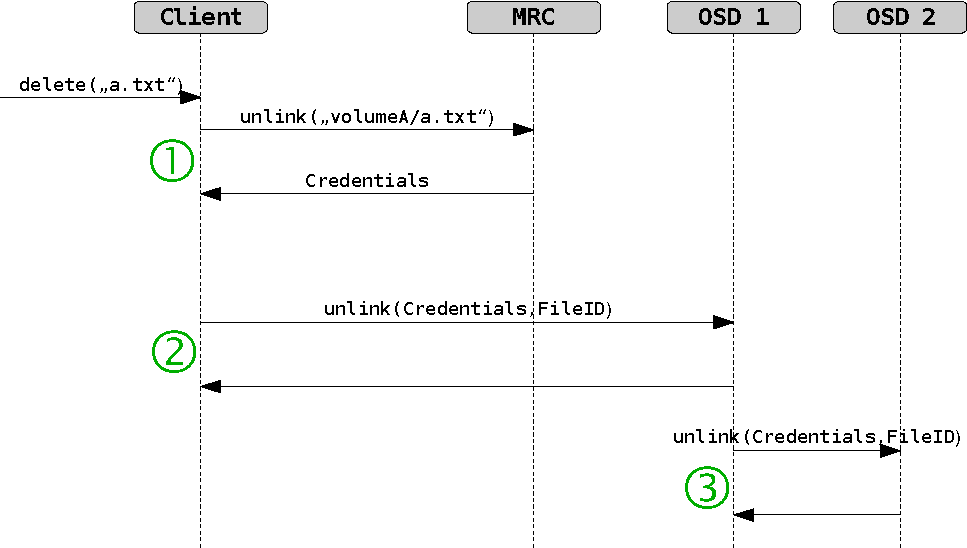
\includegraphics{images/interactions_delete.pdf}}
\caption{Deleting a file}
\label{fig:interactions_delete}
\end{figure}

\paragraph{read}

Files are read as described in the following (see Fig.\ \ref{fig:interactions_read}):

\begin{enumerate}
 \item The client receives an \texttt{open} request from the VFS. It opens the file on the MRC\index{MRC} for reading, and receives the file credentials, which contain the globally unique XtreemFS fileID, a read capability and the replica locations list.
 \item The client sends a request for reading Y bytes of data from the offset Z of the file identified by the fileID. The OSD\index{OSD} returns a buffer containing object data, as well as additional information like checksum failure notifications or padding flags.
 \item If multiple read requests are send, the client has to ensure that the capability is renewed before it times out, in order to keep the file open.
 \item The client reads more data from the file, e.g.\ another object.
 \item The client receives a \texttt{close} call. There is no need to explicitly close the file on the servers; this is implicitly done when the capabilities in the OSD\index{OSD} cache time out.
\end{enumerate}

\begin{figure}[h!]
\centering
\resizebox{0.8\width}{0.8\height}{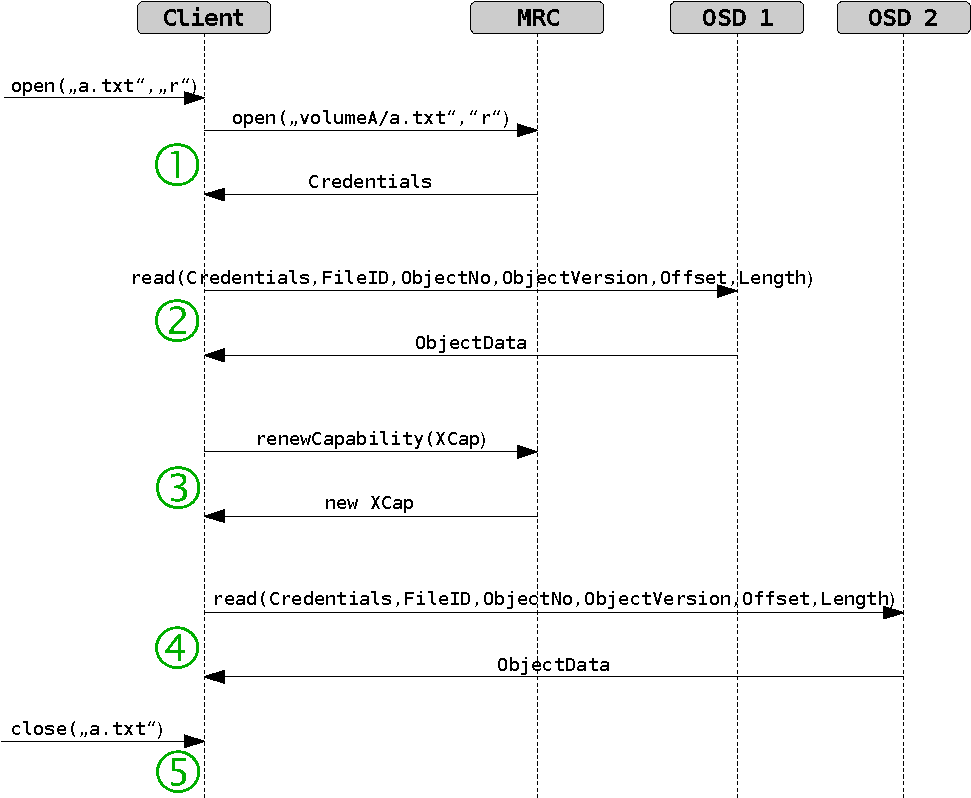
\includegraphics{images/interactions_read.pdf}}
\caption{Reading a file}
\label{fig:interactions_read}
\end{figure}

\paragraph{write}

Files are written as described in the following (see Fig.\ \ref{fig:interactions_write}):

\begin{enumerate}
 \item The client receives an \texttt{open} request from the VFS. It opens the file on the MRC\index{MRC} for writing, and receives the file credentials, which contain the globally unique XtreemFS fileID, a write capability and the replica locations list.
 \item The client sends a buffer containing the data to the OSD\index{OSD} on which the object is stored. In return, the OSD\index{OSD} sends an \texttt{OSDWriteResponse}, which must be cached and sent to the MRC\index{MRC} when the file is closed or fsync is called. The client can also decide to send pending filesize updates from time to time between capability renewals, as the lifetime of a capability can be in the range of tens of minutes.
 \item If multiple write requests are send, the client has to ensure that the capability is renewed before it times out, in order to keep the file open.
 \item The client appends data to the file by sending more \texttt{write} requests, each being answered with an \texttt{OSDWriteResponse}.
 \item The client receives a \texttt{close} call. It sends any pending \texttt{OSDWriteResponse}s to the MRC\index{MRC}, in order to update the file size. There is no need to explicitly close the file on the servers; this is implicitly done when the capabilities in the OSD\index{OSD} cache time out.
\end{enumerate}

\begin{figure}[h!]
\centering
\resizebox{0.8\width}{0.8\height}{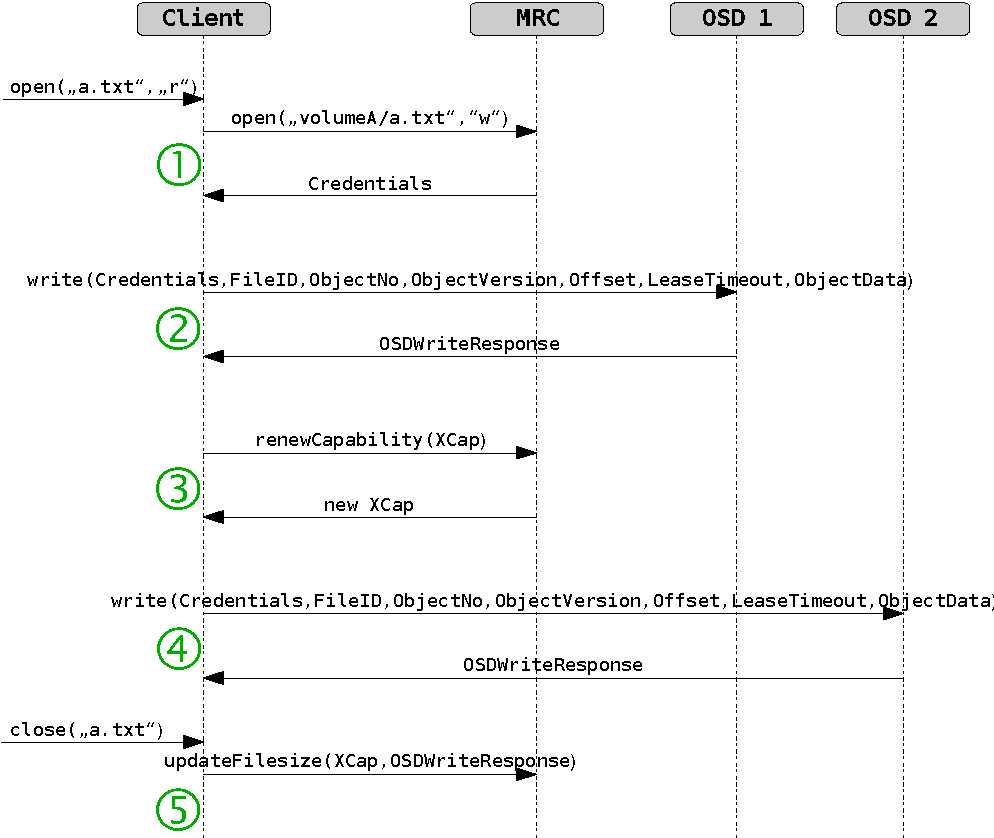
\includegraphics{images/interactions_write.pdf}}
\caption{Writing a file}
\label{fig:interactions_write}
\end{figure}

\paragraph{fsync}

Files are fsync'ed as described in the following (see Fig.\ \ref{fig:interactions_fsync}):

\begin{enumerate}
 \item The file was opened and modified.
 \item The client receives a \texttt{fsync} request from the VFS. If the file is opened all pending data will be written to the OSD\index{OSD}.
 \item The client sends any pending \texttt{OSDWriteResponse}s to the MRC\index{MRC}, in order to update the file size.
 \item The file is further modified or closed.
\end{enumerate}

\begin{figure}[h!]
\centering
\resizebox{0.8\width}{0.8\height}{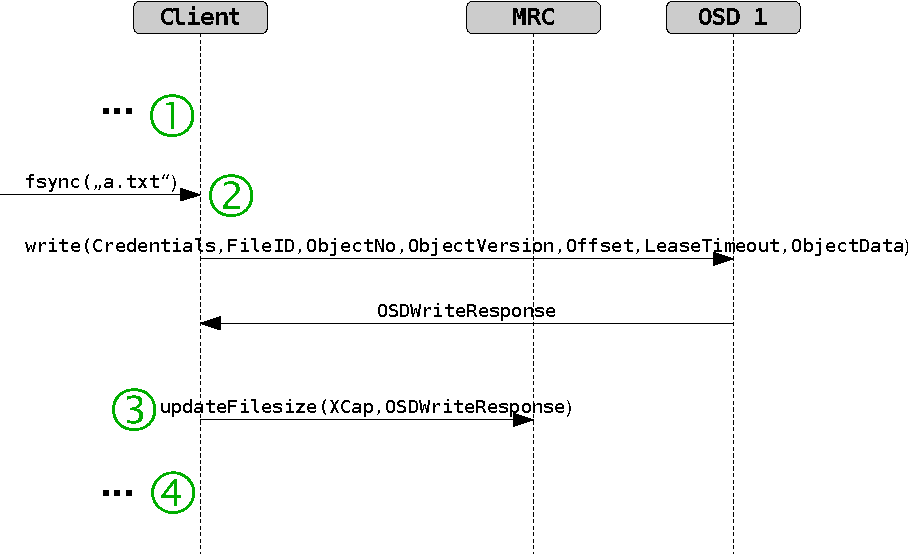
\includegraphics{images/interactions_fsync.pdf}}
\caption{Synchronizing data with the underlying device}
\label{fig:interactions_fsync}
\end{figure}

\paragraph{mkvol}

New volumes are created as described in the following (see Fig.\ \ref{fig:interactions_mkvol}):

\begin{enumerate}
 \item The client receives an \texttt{mkvol} request. In response, it creates the volume on the MRC\index{MRC}.
 \item The MRC\index{MRC} registers the volume at the DIR\index{DIR}.
 \item If no problems occur, the MRC\index{MRC} responds to the client with an acknowledgment.
\end{enumerate}

\begin{figure}[h!]
\centering
\resizebox{0.8\width}{0.8\height}{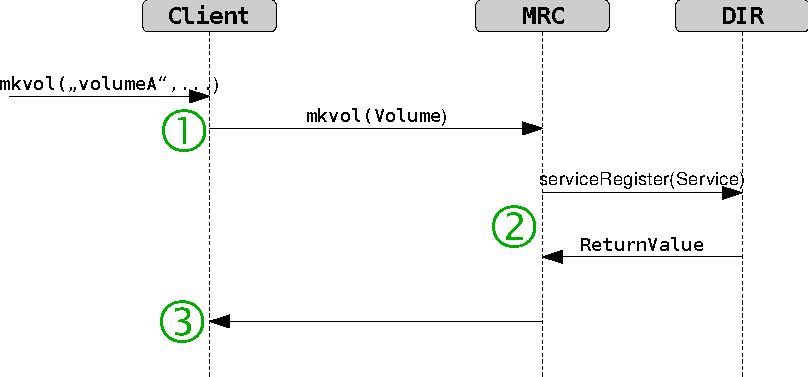
\includegraphics{images/interactions_mkvol.pdf}}
\caption{Creating a new volume}
\label{fig:interactions_mkvol}
\end{figure}

\paragraph{rmvol}

Volumes are deleted as described in the following (see Fig.\ \ref{fig:interactions_rmvol}):

\begin{enumerate}
 \item The client receives a \texttt{rmvol} request from the console. In response, it removes the volume on the MRC\index{MRC}.
 \item The MRC\index{MRC} deregisters the volume at the DIR\index{DIR}.
 \item If no problems occur, the MRC\index{MRC} responds to the client with an acknowledgment.
\end{enumerate}

\begin{figure}[h!]
\centering
\resizebox{0.8\width}{0.8\height}{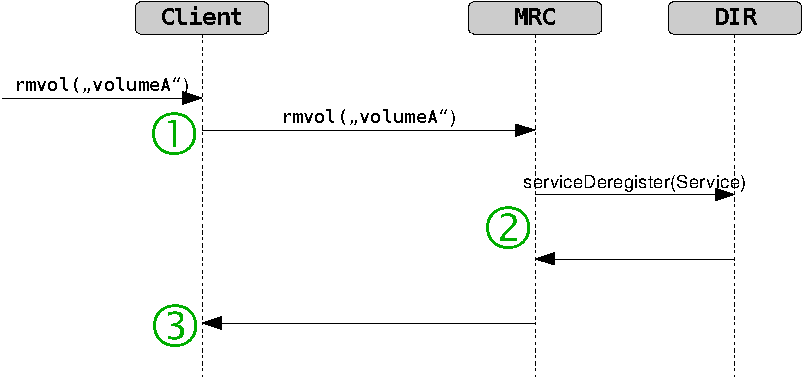
\includegraphics{images/interactions_rmvol.pdf}}
\caption{Deleting an existing volume}
\label{fig:interactions_rmvol}
\end{figure}

\paragraph{removeReplica}

Single replicas of a file are deleted as described in the following (see Fig.\ \ref{fig:interactions_rmrepl}):

\begin{enumerate}
 \item The client receives a \texttt{removeReplica} request from the console. It sends a request to the MRC\index{MRC} to remove the replica with a matching head OSD\index{OSD}. In response, it receives the file credentials, which contain the globally unique XtreemFS fileID, a deletion capability and the list of replica locations.
 \item The client initiates the deletion of the replica's file content by invoking the \texttt{unlink} operation on the head OSD\index{OSD} (i.e.\ the first OSD\index{OSD} of a stripe).
 \item The head OSD\index{OSD} delays the deletion until all clients have closed the file, i.e.\ all capabilities known to the head OSD\index{OSD} have timed out. In turn, the head OSD\index{OSD} initiates the deletion of file objects on the remaining OSDs via \texttt{unlink}.
 \item If a client finds out that its replica locations list for the file is outdated, it has to retrieve the new replica locations list from the MRC\index{MRC}.
\end{enumerate}

\begin{figure}[h!]
\centering
\resizebox{0.8\width}{0.8\height}{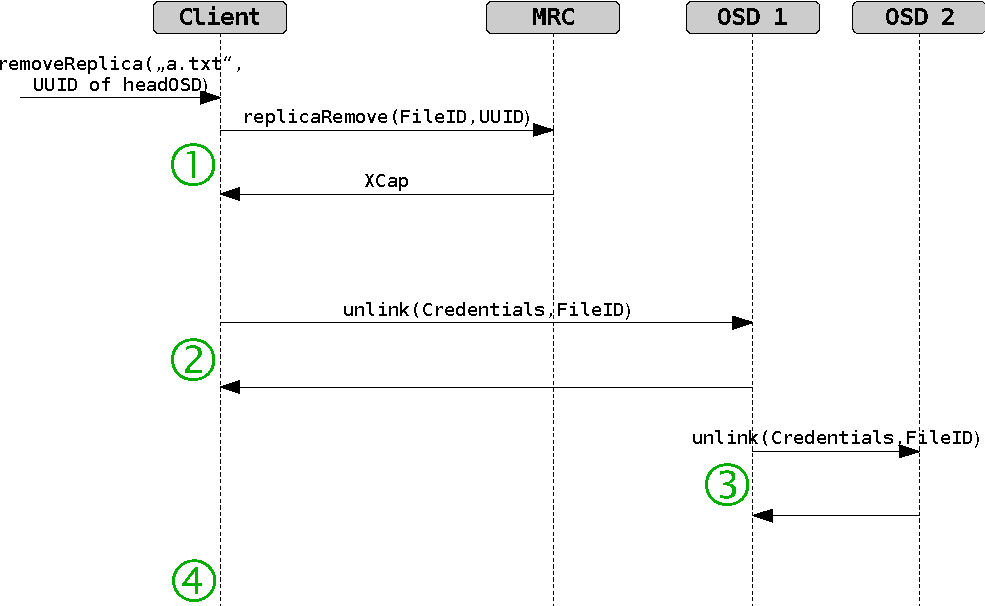
\includegraphics{images/interactions_rmrepl.pdf}}
\caption{Deleting a replica of a file}
\label{fig:interactions_rmrepl}
\end{figure}

\printindex

\bibliographystyle{plain}
\bibliography{bib}

\end{document}
